\chapter{Análisis de la Infraestructura Eléctrica y Mapeo de Señales}
\lineaLateral

\begin{resumenCapitulo}
	Este capítulo detalla la ingeniería inversa aplicada a la infraestructura electrónica del robot ante la ausencia de documentación original. Se sistematizó el mapeo del cableado, clasificando señales de potencia, encoders y finales de carrera, e identificando discrepancias en el código de colores. Esta caracterización técnica es el fundamento para el diseño de la PCB de acondicionamiento y la integración con la tarjeta externa.
\end{resumenCapitulo}


\section{Distribución Espacial del Hardware y Configuración de Periféricos}

Para garantizar la integridad mecánica del brazo \textit{Mitsubishi RV-M1} durante las pruebas de movimiento, se realizó una auditoría técnica de la ubicación de cada componente crítico. Esta inspección fue fundamental, dado que el estado físico de los actuadores y sensores determina los límites de operación segura del sistema.

Como se detalla en la Figura \ref{fig:ubicacion}, la arquitectura del robot distribuye los cinco grados de libertad (J1 a J5) junto con sus respectivos elementos de seguridad y retroalimentación. La inspección física permitió confirmar la siguiente disposición de componentes:

\begin{itemize}
	\item \textbf{Actuadores y Frenos:} Los ejes de mayor carga (J2 y J3) cuentan con frenos electromecánicos dedicados para evitar el colapso del brazo ante una pérdida de energía accidental.
	\item \textbf{Sistema de Retroalimentación (Encoders):} Se verificó que los encoders se encuentran acoplados directamente a cada actuador. Físicamente, estos se ubican en la sección posterior de los motores, resguardados por una tapa que protege el disco ranurado y la electrónica de lectura, facilitando una medición directa de la posición del eje.
	\item \textbf{Finales de Carrera:} Se identificó la posición estratégica de los interruptores de límite (\textit{limit switches}) en cada eje, los cuales actúan como la última línea de defensa ante sobre-recorridos mecánicos.
\end{itemize}


\begin{figure}[h]
	\centering
	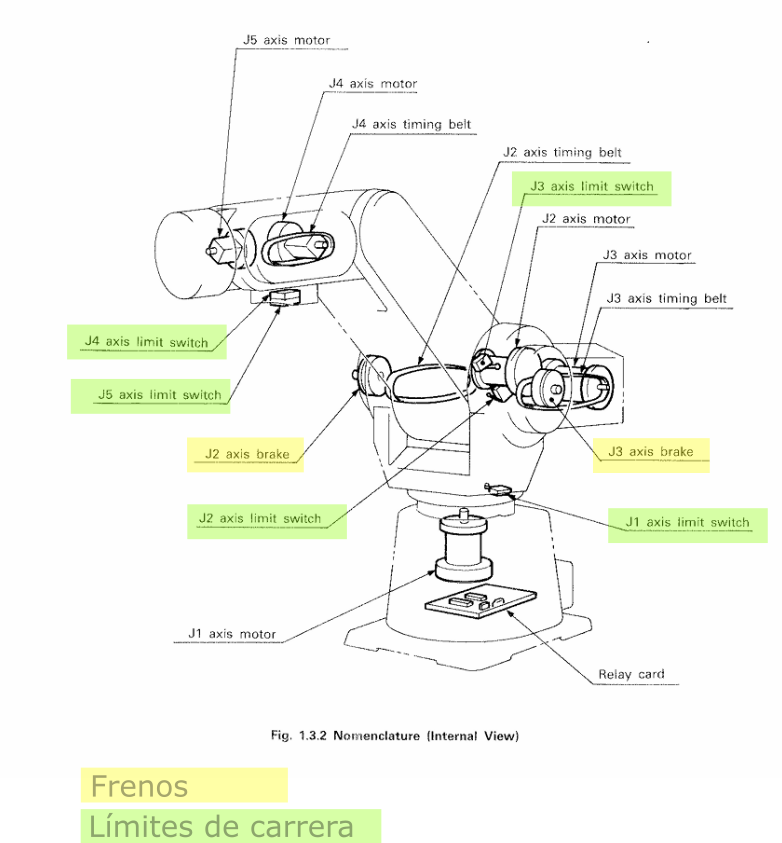
\includegraphics[width=1\linewidth]{images/Infraestructura/ubicaciobn}
	\caption[Distribución interna de actuadores y periféricos]{Nomenclatura y ubicación física de motores (J1-J5), frenos electromecánicos y sensores de límite de carrera del Mitsubishi RV-M1.}
	\label{fig:ubicacion}
\end{figure}

\begin{figure}[htbp]
	\centering
	% Título del bloque de seguridad (Llave cerrada correctamente al final de la línea)
	{\large \textbf{Registro fotográfico de los finales de Carrera}} \\[0.3cm]
	
	% --- FILA 1: LS1 y LS2 ---
	\begin{minipage}{0.48\textwidth}
		\centering
		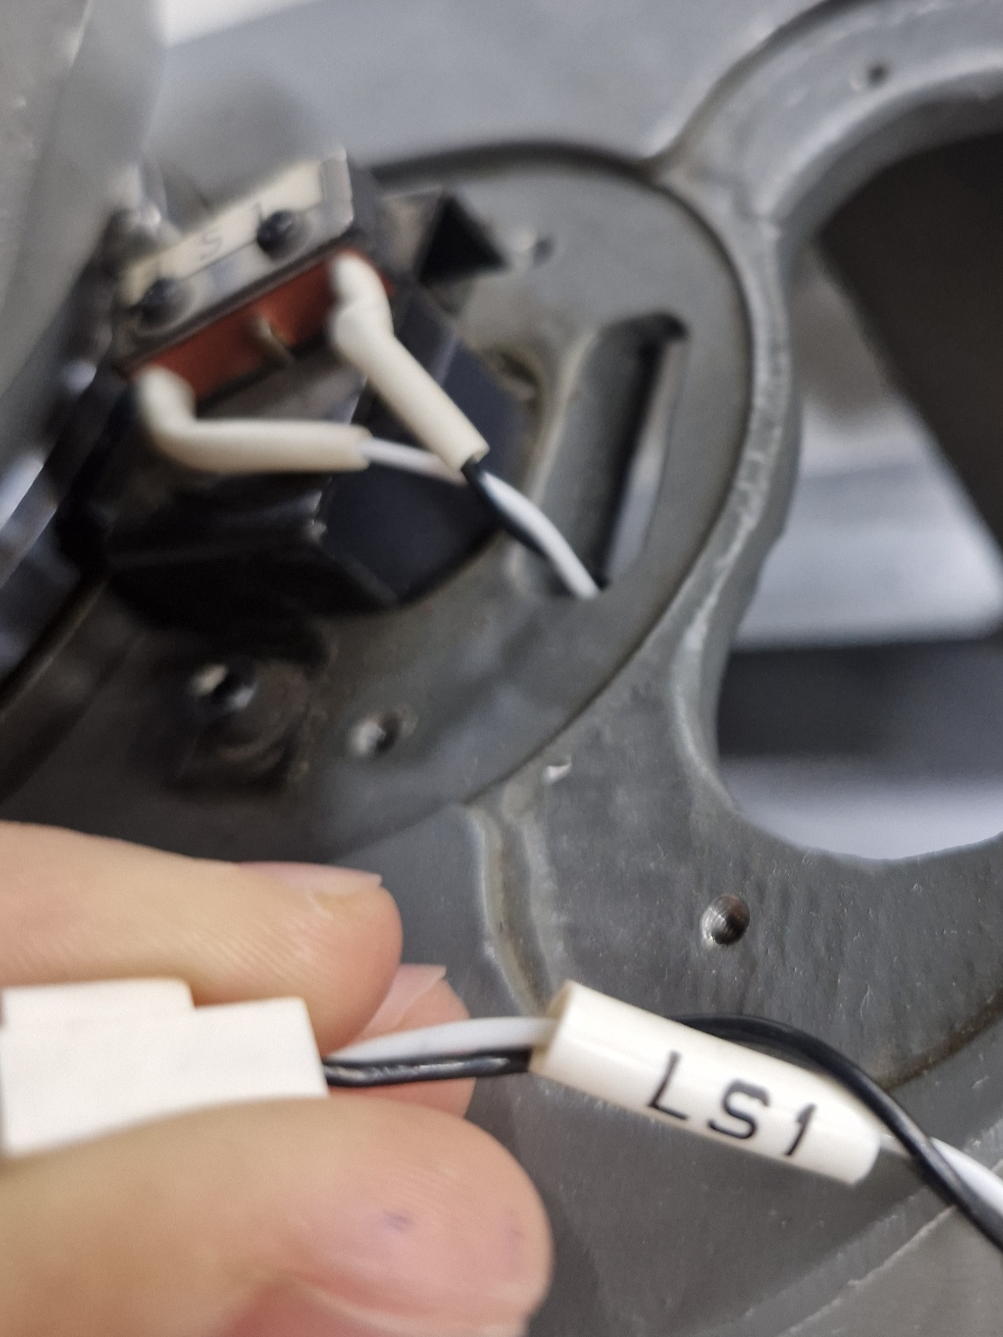
\includegraphics[width=0.85\linewidth]{images/Infraestructura/ls1.png}
		\caption[Ubicación de LS1]{\small Ubicación física del sensor de límite LS1.}
		\label{fig:ls1_inspeccion}
	\end{minipage}
	\hfill
	\begin{minipage}{0.48\textwidth}
		\centering
		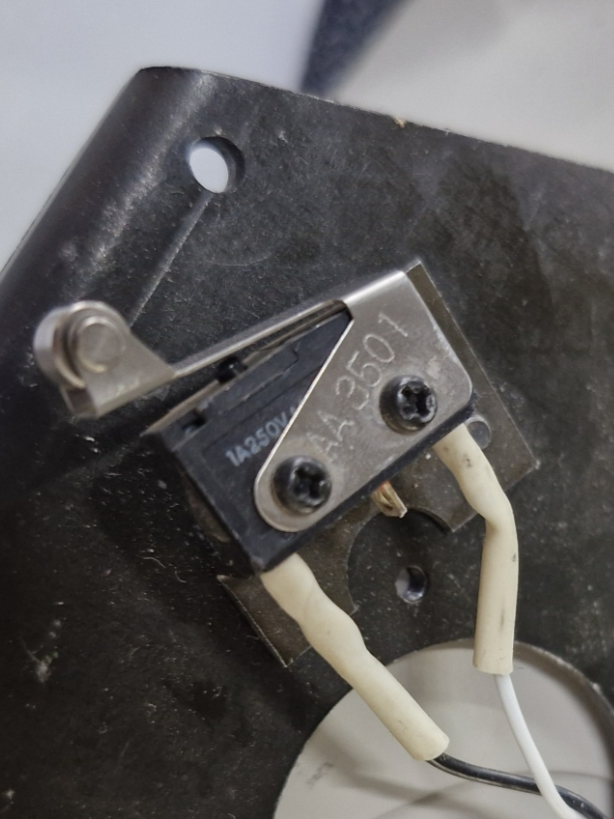
\includegraphics[width=0.85\linewidth]{images/Infraestructura/ls2ubic.png}
		\caption[Ubicación de LS2]{\small Detalle del componente LS2.}
		\label{fig:ls2_inspeccion}
	\end{minipage}
	
	\vspace{0.4cm} % Espacio vertical entre filas
	
	% --- FILA 2: LS3 y LS4/LS5 ---
	\begin{minipage}{0.48\textwidth}
		\centering
		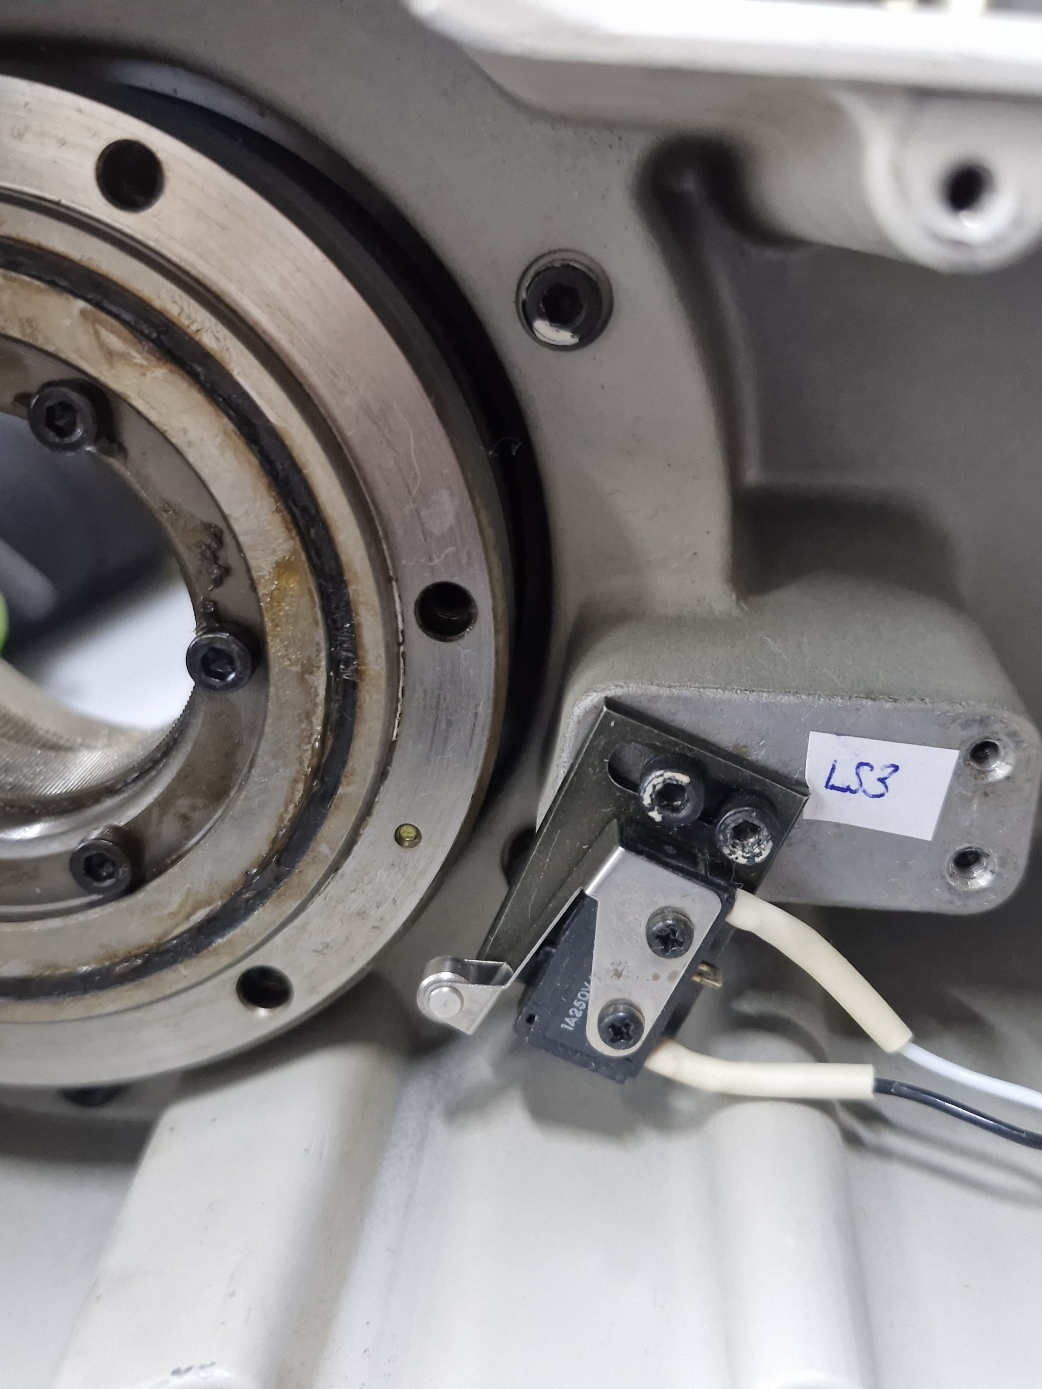
\includegraphics[width=0.85\linewidth]{images/Infraestructura/ls3ubica.png}
		\caption[Ubicación de LS3]{\small Ubicación física del sensor de límite LS3.}
		\label{fig:ls3_inspeccion}
	\end{minipage}
	\hfill
	\begin{minipage}{0.48\textwidth}
		\centering
		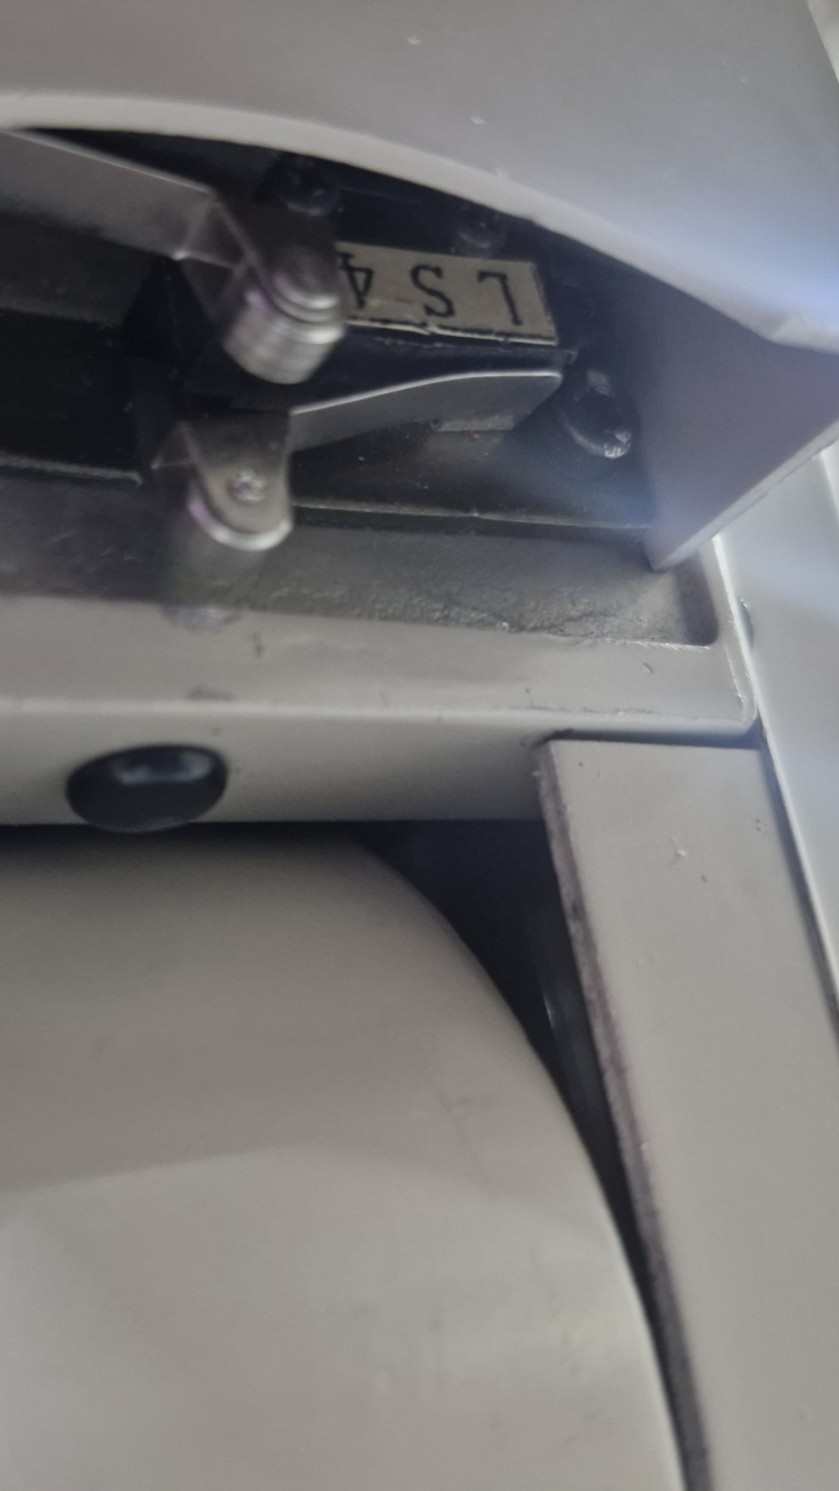
\includegraphics[width=0.65\linewidth]{images/Infraestructura/ls4ls5.jpg}
		\caption[Ubicación de LS4 y LS5]{\small Sensores de límite correspondientes a los ejes terminales.}
		\label{fig:ls4ls5_inspeccion}
	\end{minipage}
\end{figure}
	
	
	\begin{figure}[h]
		\centering
		% Título opcional para el bloque de actuadores
		{\large \textbf{Registro fotográfico  de los Motores DC}} \\[0.3cm] 
		
		% --- LADO IZQUIERDO: Motor Muñeca ---
		\begin{minipage}{0.48\textwidth}
			\centering
			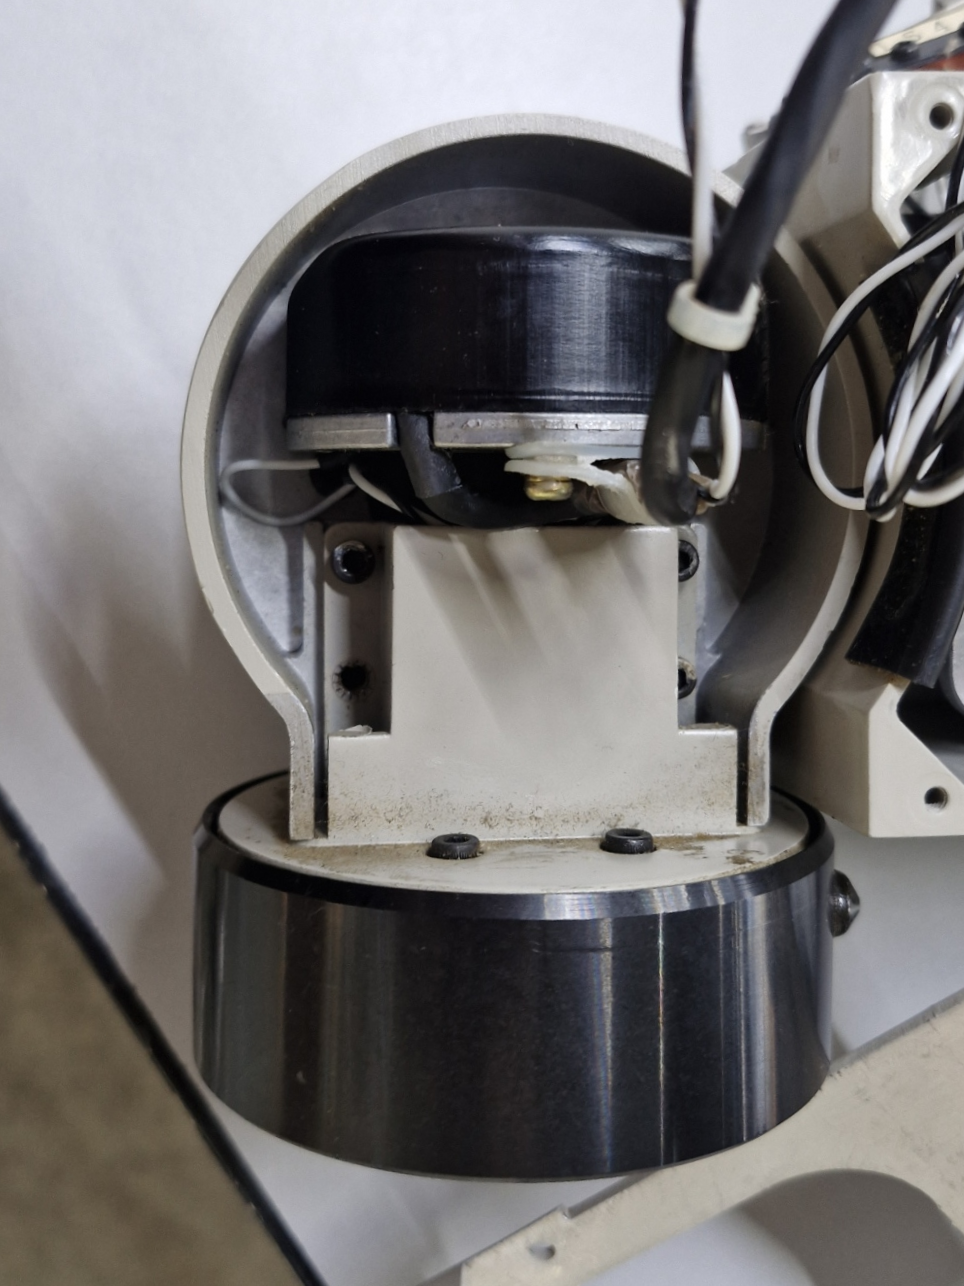
\includegraphics[width=0.70\linewidth]{images/Infraestructura/motorMuneca.png}
			\caption[Motor de la muñeca]{\small Detalle del motor correspondiente a la articulación de la muñeca.}
			\label{fig:mmuneca}
		\end{minipage}
		\hfill
		% --- LADO DERECHO: Motor Hombro/Antebrazo ---
		\begin{minipage}{0.48\textwidth}
			\centering
			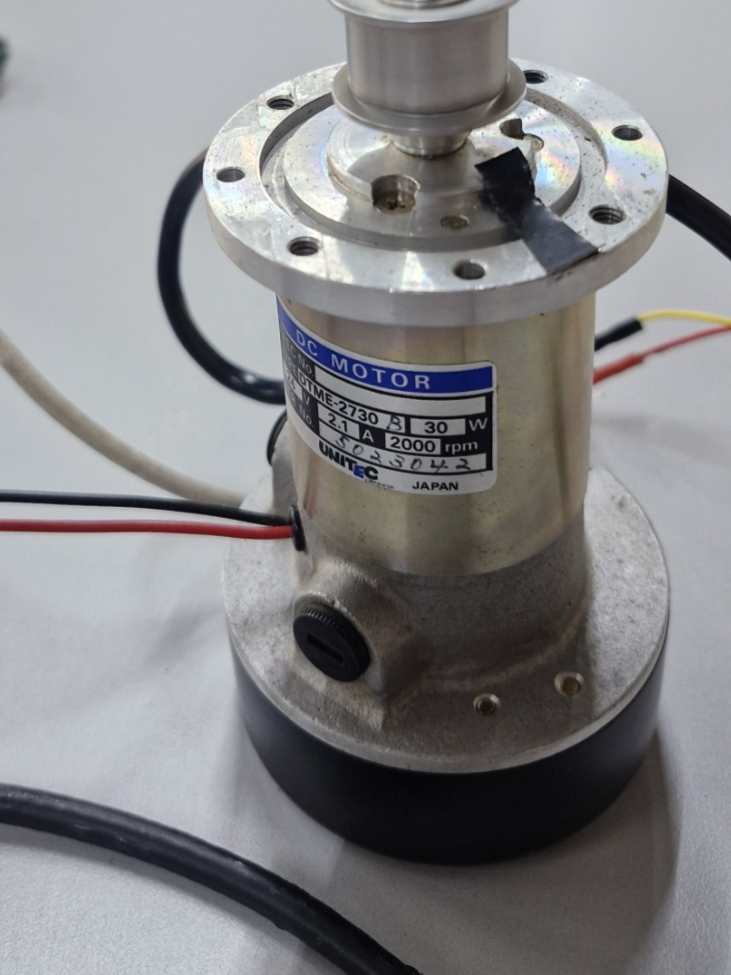
\includegraphics[width=0.70\linewidth]{images/Infraestructura/motor.png}
			\caption[Motor hombro/antebrazo]{\small Configuración de los motores de hombro y antebrazo.}
			\label{fig:mhombroantebrazo}
		\end{minipage}
		
		\vspace{0.5cm} % Espacio para que el bloque "respire" y no se pegue al texto inferior
	\end{figure}
	
	\clearpage
	\section{Topología Física y Distribución de Componentes}
	Para comprender la conectividad del brazo robótico, se definieron tres conceptos fundamentales que clasifican la ruta de las señales desde el sensor hasta el controlador final:
	
	\renewcommand{\arraystretch}{1.5}
	
	\begin{table}[h]
		\centering
		\caption[Definiciones del sistema de interconexión]{Jerarquía y conceptos del sistema de cableado del brazo robótico.}
		\label{tab:conceptos_cableado}
		\renewcommand{\arraystretch}{1.5}
		
		% Cambiamos a green!10 para que sea un verde más definido y no parezca crema/amarillo
		\rowcolors{2}{green!10}{white}
		
		\begin{tabular}{>{\raggedright\arraybackslash\bfseries}p{4.5cm} p{9cm}}
			\toprule
			% Encabezado limpio (blanco)
			\textbf{Concepto} & \textbf{Descripción Técnica} \\ \midrule
			Segmento de Captación & Conductores integrados directamente en la carcasa de cada periférico (encoders/motores). \\
			Segmento de Transmisión & Arnés intermedio que vincula la captación con la terminal del cable umbilical. \\
			Interfaz SDP & Punto de consolidación central para las señales de retroalimentación, frenado y seguridad. \\
			\bottomrule
		\end{tabular}
	\end{table}
	
	\vspace{0.5 in}
	\begin{figure}[h]
		\centering
		% Título del bloque para dar contexto a la jerarquía
		{\large \textbf{Jerarquía del Sistema de Cableado: Segmentos A, B y C}} \\[0.3cm] 
		
		% --- 1. Segmento de Captación ---
		\begin{minipage}{0.32\textwidth}
			\centering
			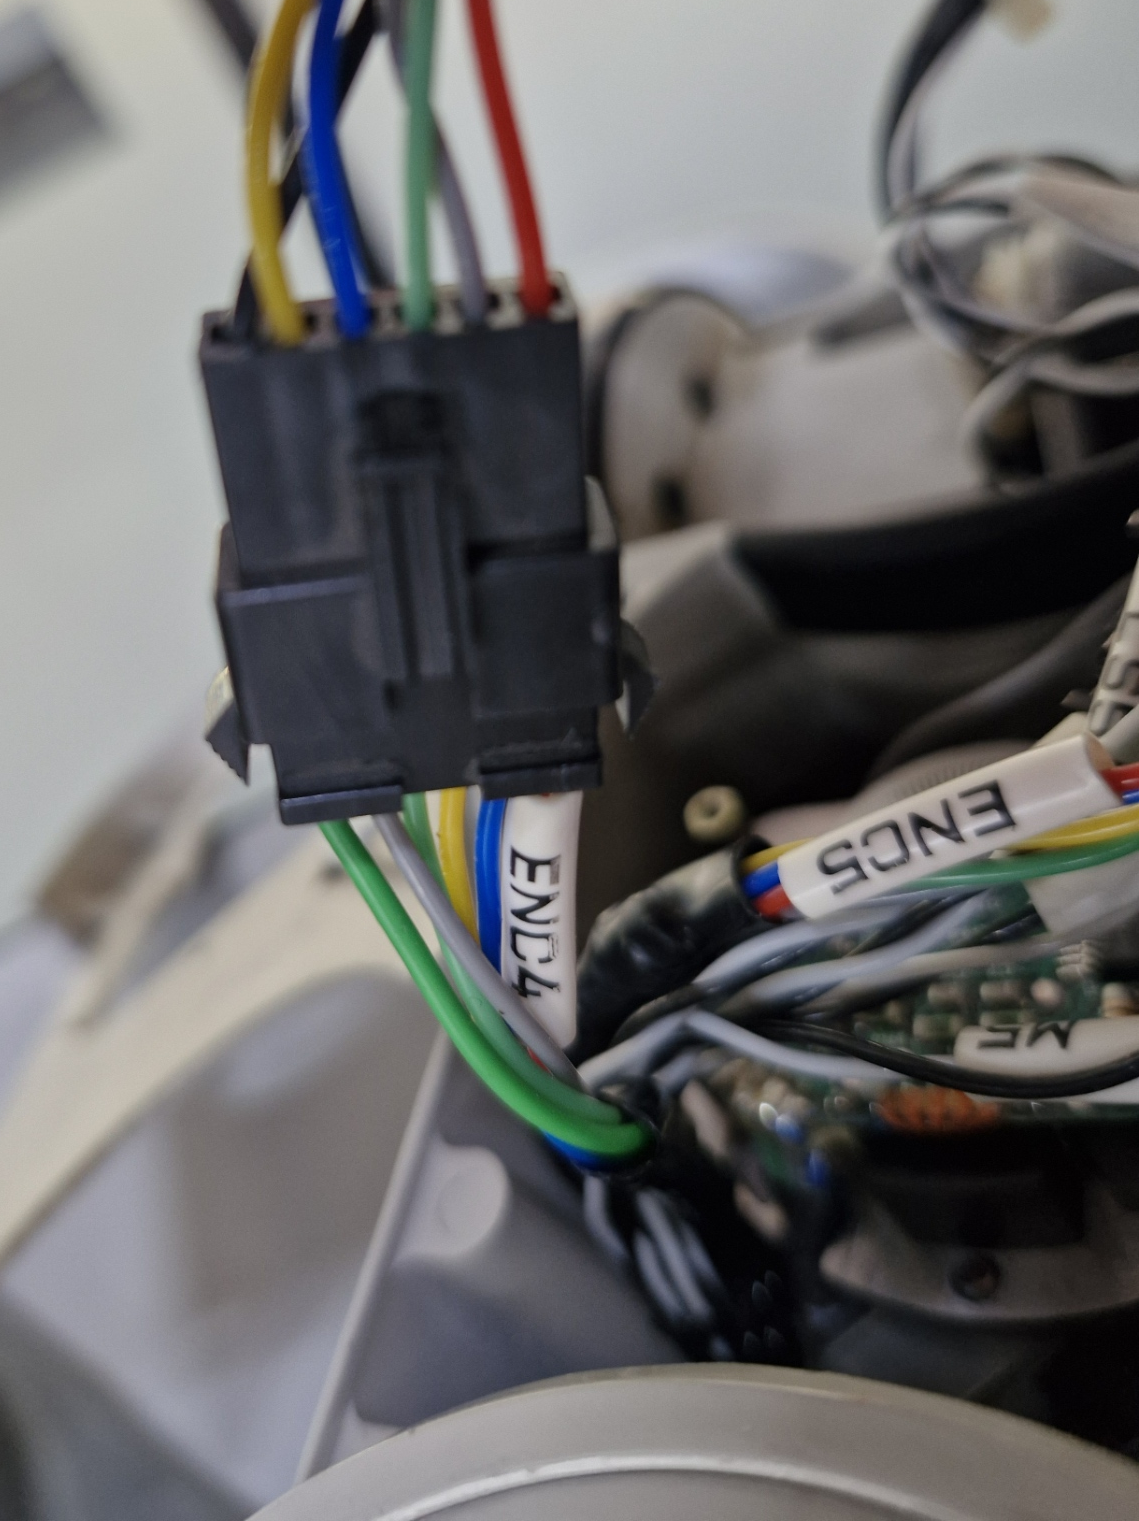
\includegraphics[width=0.95\linewidth]{images/Infraestructura/segCaptacion.png}
			\caption[Segmento de captación]{\small Segmento de captación.}
			\label{fig:captacionseg}
		\end{minipage}
		\hfill
		% --- 2. Segmento de Transmisión ---
		\begin{minipage}{0.32\textwidth}
			\centering
			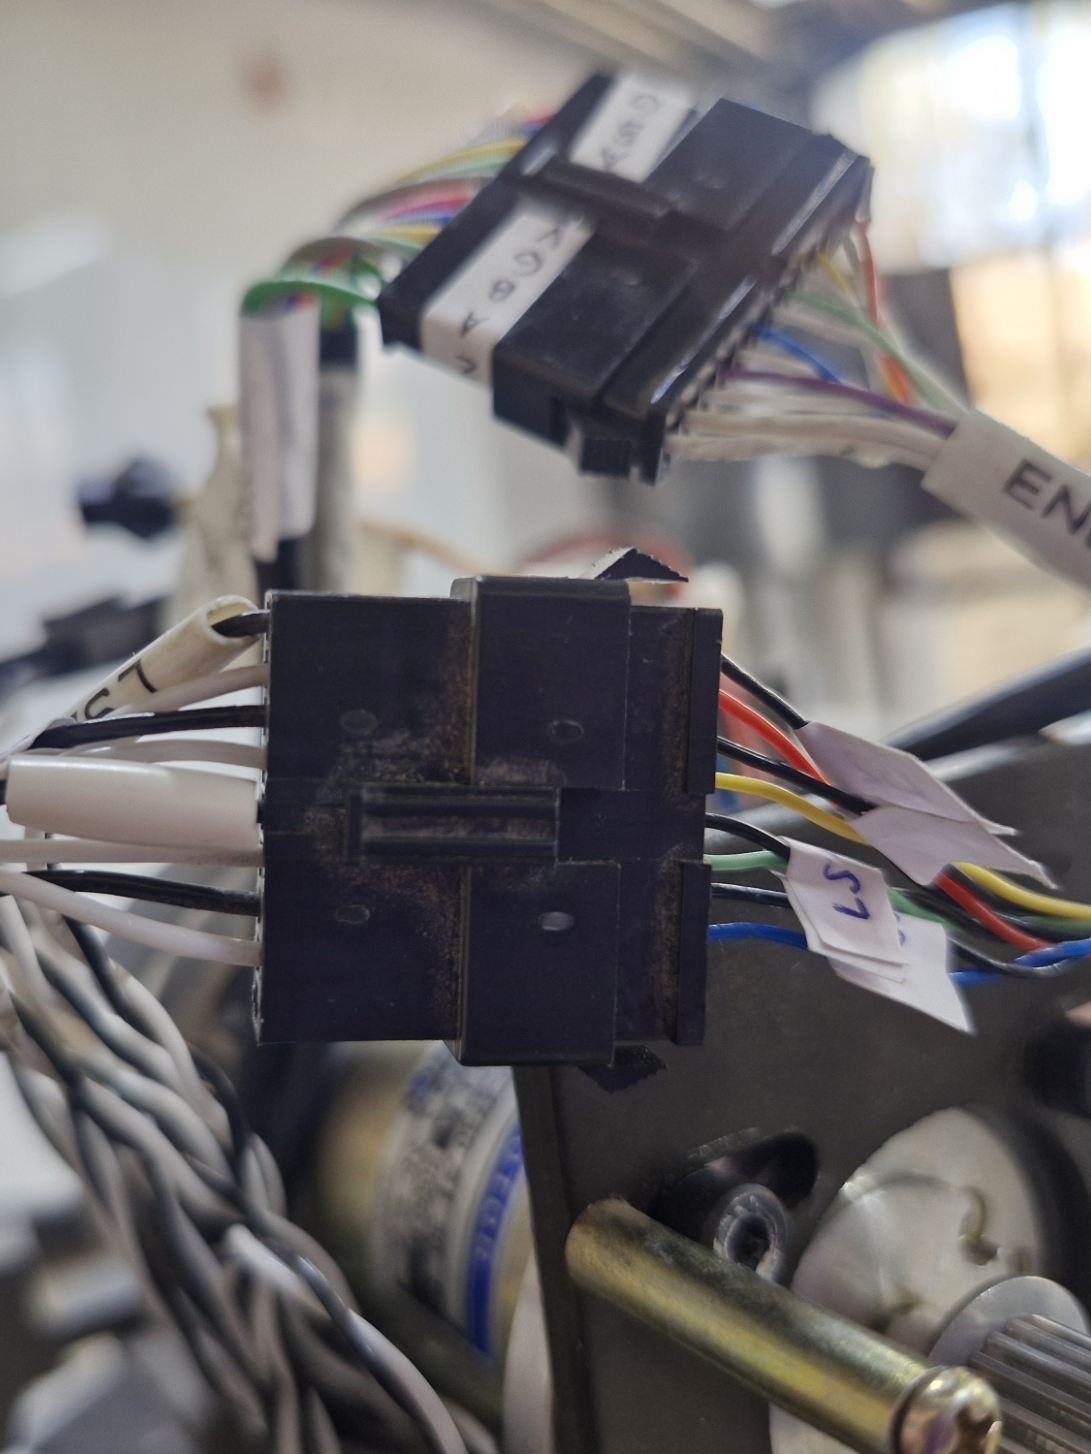
\includegraphics[width=0.95\linewidth]{images/Infraestructura/SegmentoTrasmision.png}
			\caption[Segmento de transmisión]{\small Segmento de transmisión.}
			\label{fig:SegmentoTrasmision}
		\end{minipage}
		\hfill
		% --- 3. Segmento SDP ---
		\begin{minipage}{0.32\textwidth}
			\centering
			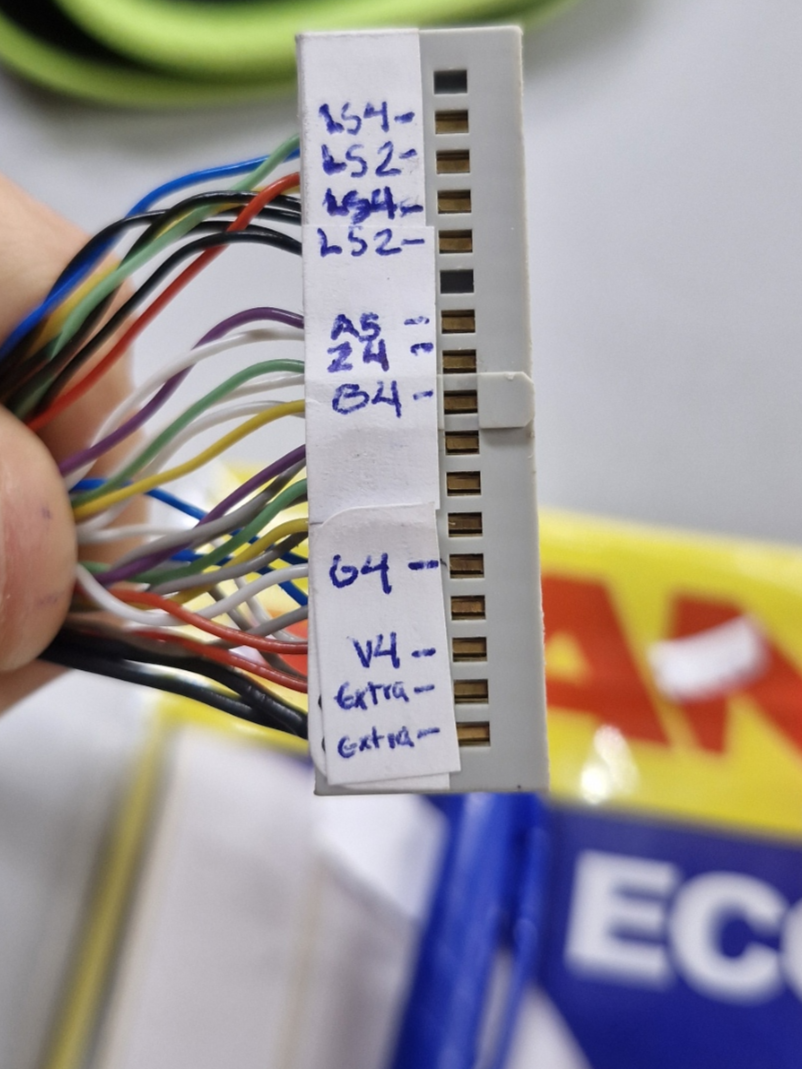
\includegraphics[width=0.95\linewidth]{images/Infraestructura/sdsssd.png}
			\caption[Segmento SDP]{\small Segmento SDP.}
			\label{fig:sdp_interfaz}
		\end{minipage}
		
		\vspace{0.4cm} % Espacio inferior para separar del siguiente párrafo
	\end{figure}
	\clearpage
	\section{Jerarquía del Sistema de Interconexión}
	El cable principal de comunicación, se divide en dos secciones lógicas para segregar potencia y control. El estudio de este componente permitió identificar el estado físico de los conectores y sus requerimientos técnicos:
	
	\begin{itemize}
		\item \textbf{Segmento A:} Destinado exclusivamente a la potencia de motores y el accionamiento de frenos.
		\item \textbf{Segmento B:} Consiste en una terminal de $2 \times 17$ pines que centraliza los datos de los encoders y los interruptores de final de carrera.
	\end{itemize}
	
	
	\begin{figure}[h]
		\centering
		% Título del bloque dentro de la figura
		{\large \textbf{SDP del Segmento A}} \\[0.3cm] 
		
		% --- FILA 1 ---
		\begin{minipage}{0.45\textwidth}
			\centering
			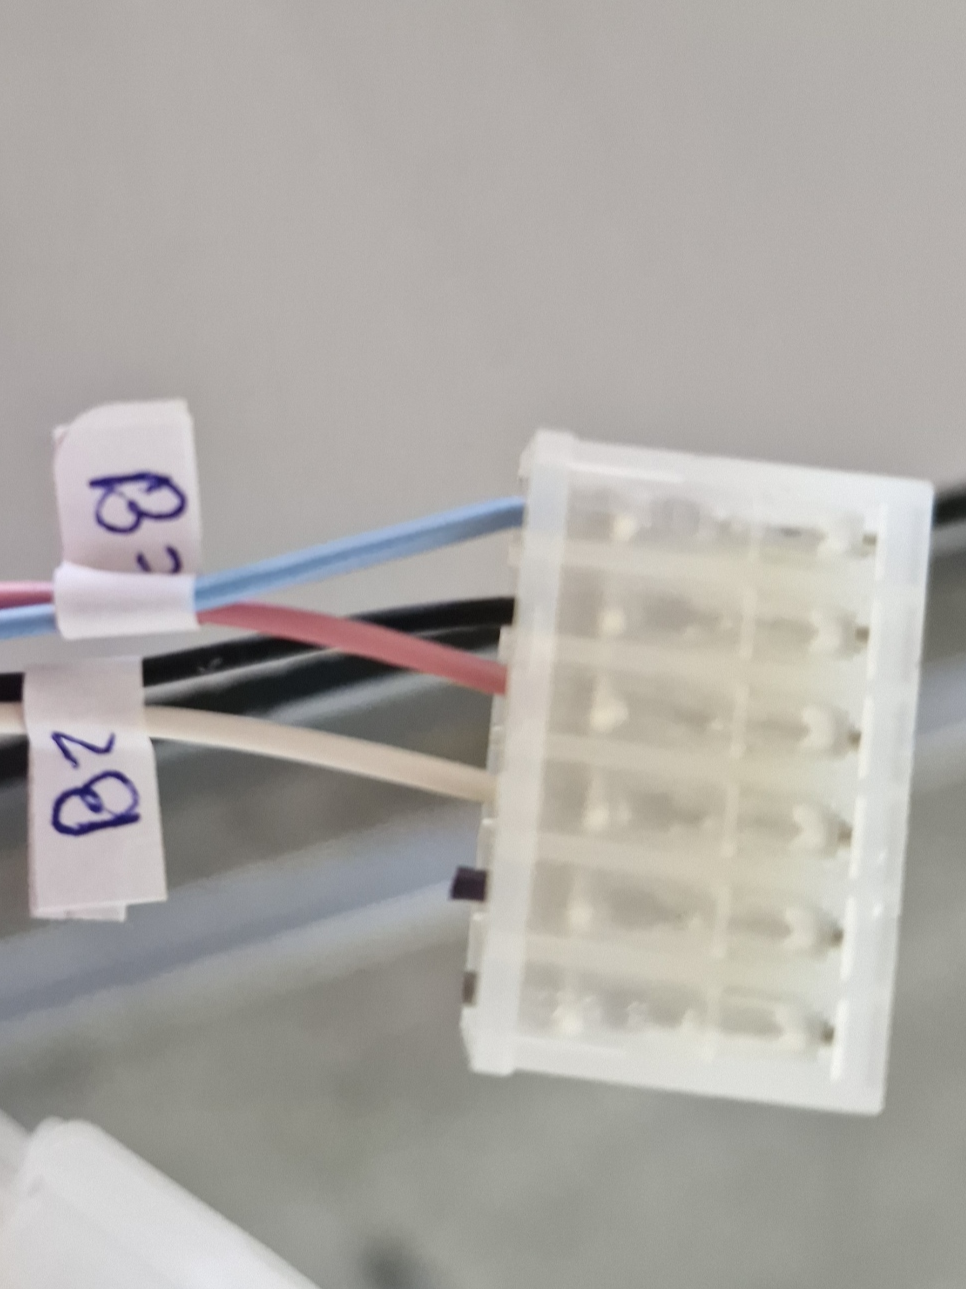
\includegraphics[width=0.75\linewidth]{images/Infraestructura/FrenosT.png}
			\caption[SDP de frenos]{\small SDP de los frenos.}
			\label{fig:frenos_sdp}
		\end{minipage}
		\hfill
		\begin{minipage}{0.45\textwidth}
			\centering
			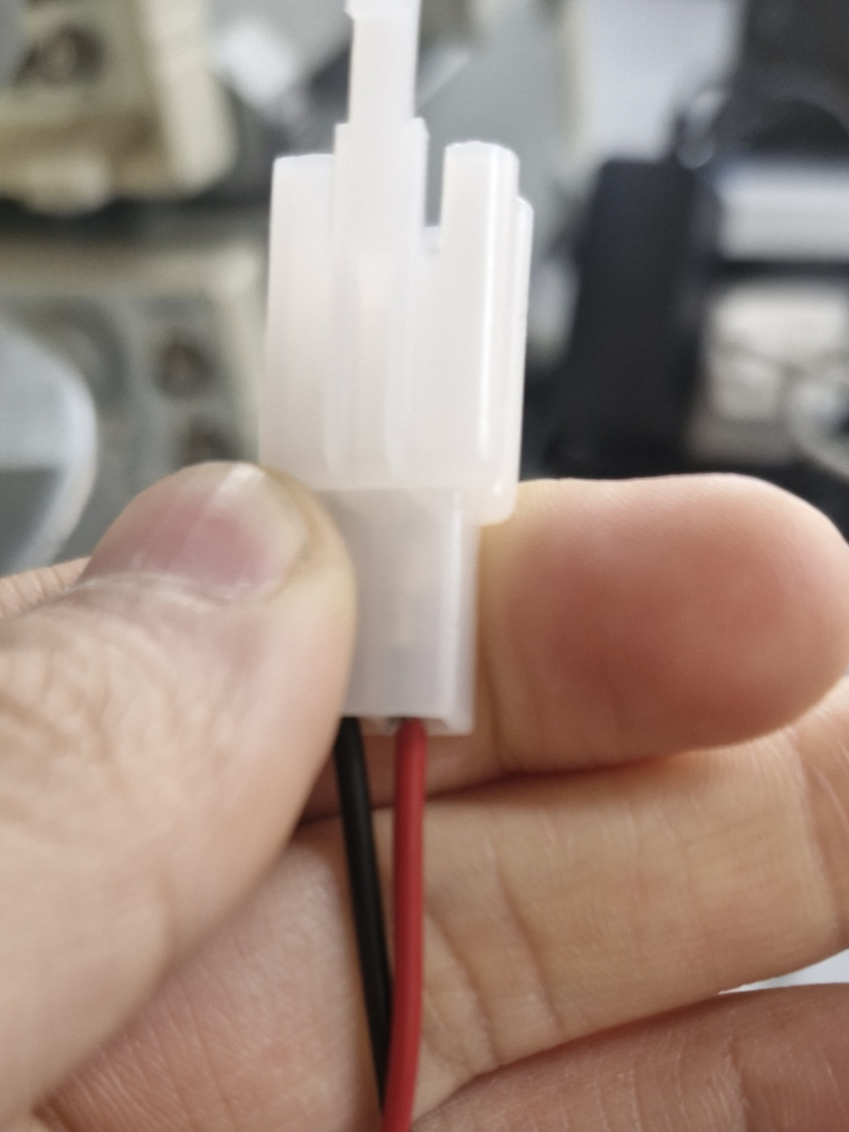
\includegraphics[width=0.75\linewidth]{images/Infraestructura/m1t.png}
			\caption[SDP de M1]{\small SDP de M1.}
			\label{fig:m1ter}
		\end{minipage}
		
		\vspace{0.2cm} % Espacio entre filas
		
		% --- FILA 2 ---
		\begin{minipage}{0.45\textwidth}
			\centering
			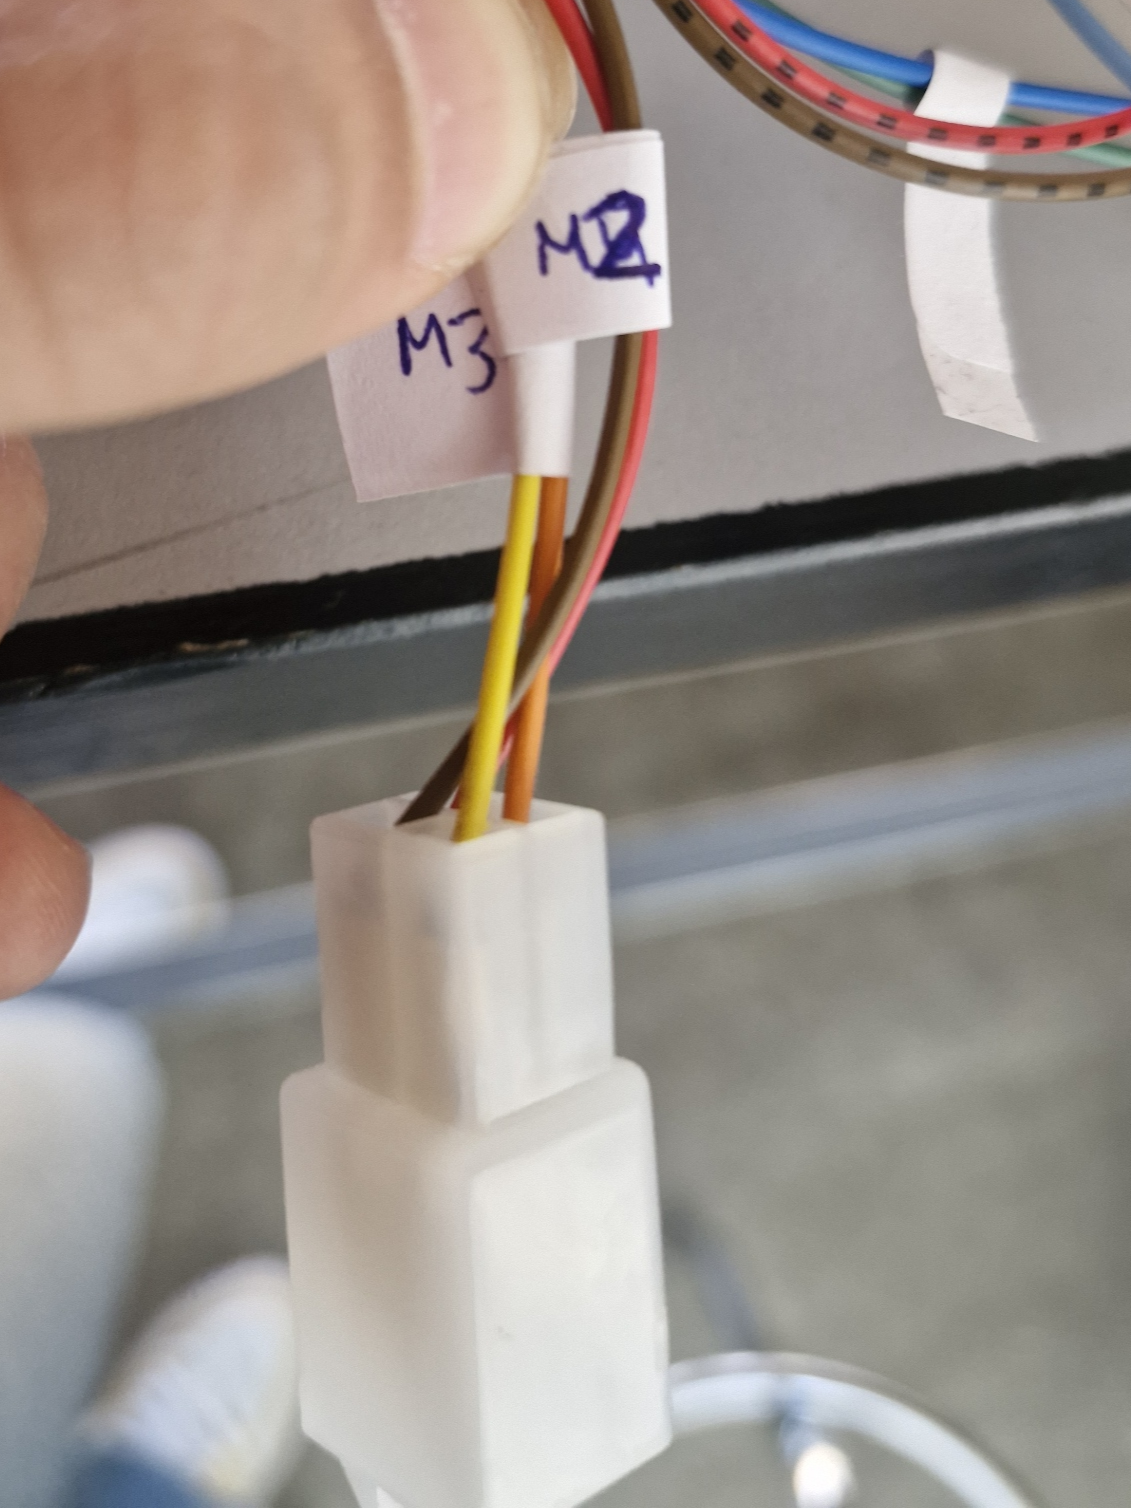
\includegraphics[width=0.75\linewidth]{images/Infraestructura/SDPM3M2.png}
			\caption[SDP de M2/M3]{\small SDP de M2 y M3.}
			\label{fig:m3m2ter}
		\end{minipage}
		\hfill
		\begin{minipage}{0.45\textwidth}
			\centering
			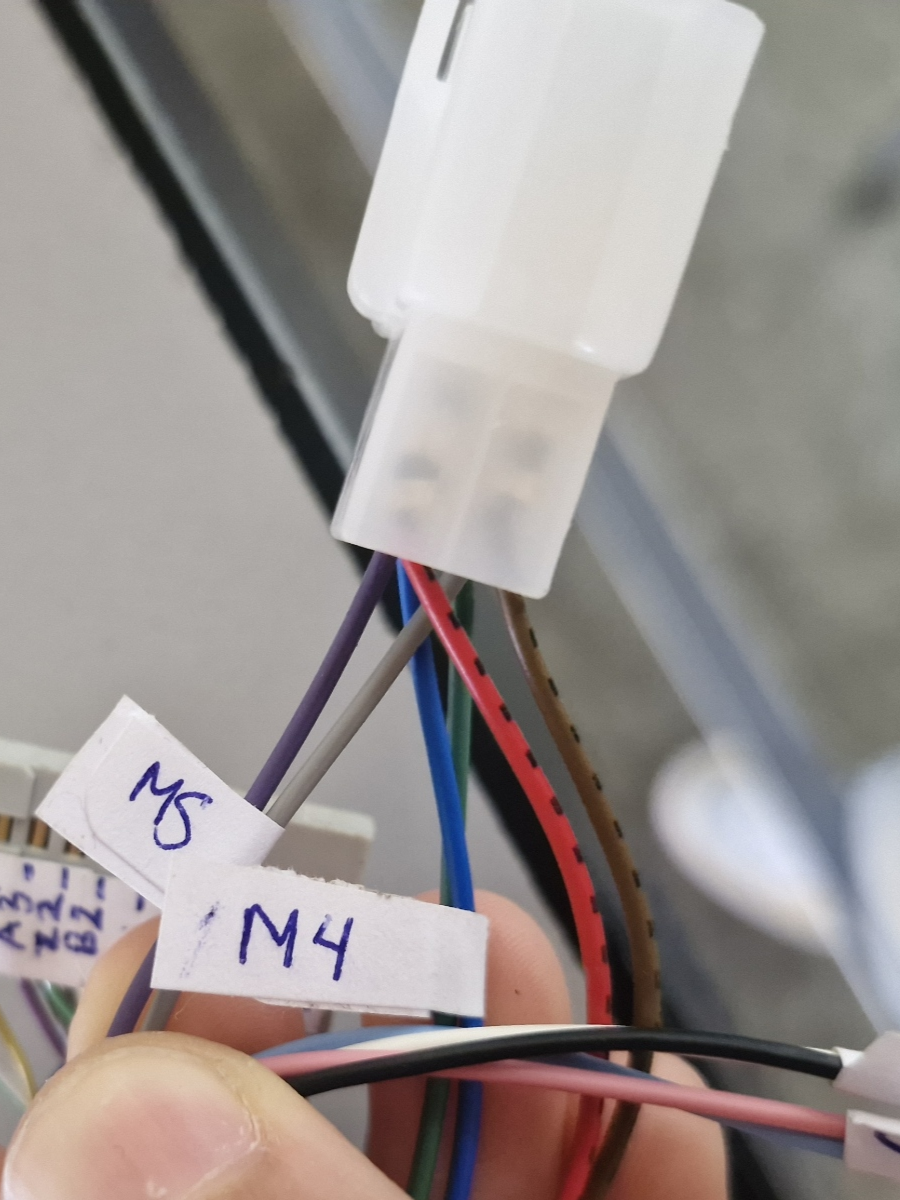
\includegraphics[width=0.75\linewidth]{images/Infraestructura/m5m4t.png}
			\caption[SDP de M4/M5]{\small SDP de M4 y M5.}
			\label{fig:m4m5ter}
		\end{minipage}
	\end{figure}
	
	\begin{figure}[h]
		\centering
		{\large \textbf{SDP del Segmento B}} \\[0.3cm] 
		% --- LADO IZQUIERDO: SEGMENTO B ---
		\begin{minipage}{0.48\textwidth}
			\centering
			\textbf{Segmento B (Izquierda)} \\ [0.2cm]
			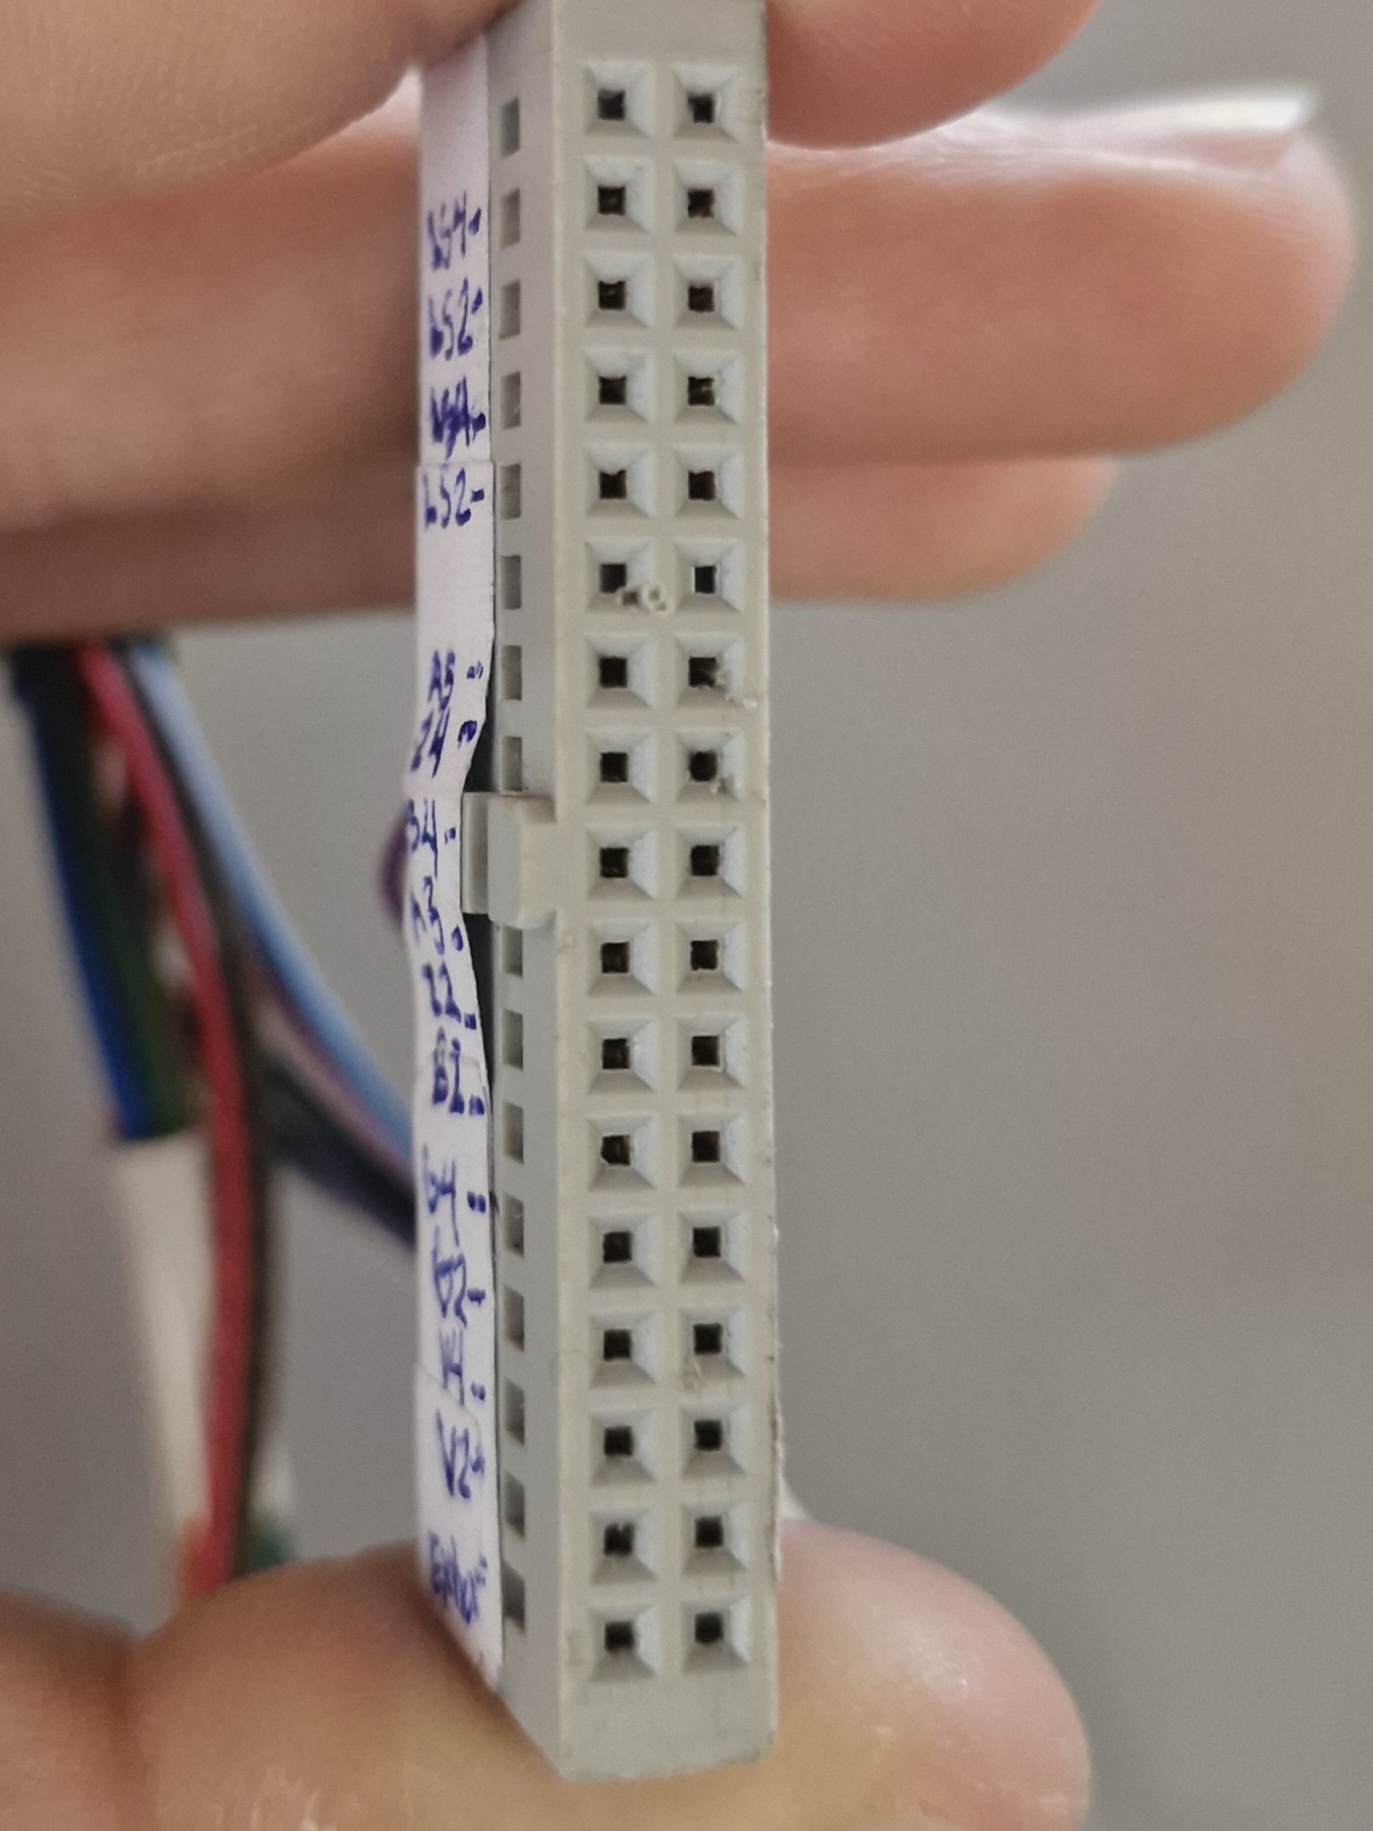
\includegraphics[width=0.95\linewidth]{images/Infraestructura/sdpTerminalA.png}
			\caption[SDP del segmento B]{\small Detalle técnico del SDP correspondiente al segmento B.}
			\label{fig:sdp_seg_b}
		\end{minipage}
		\hfill
		% --- LADO DERECHO: DISTRIBUCIÓN GENERAL ---
		\begin{minipage}{0.48\textwidth}
			\centering
			\textbf{Distribución de Segmentos} \\ [0.2cm]
			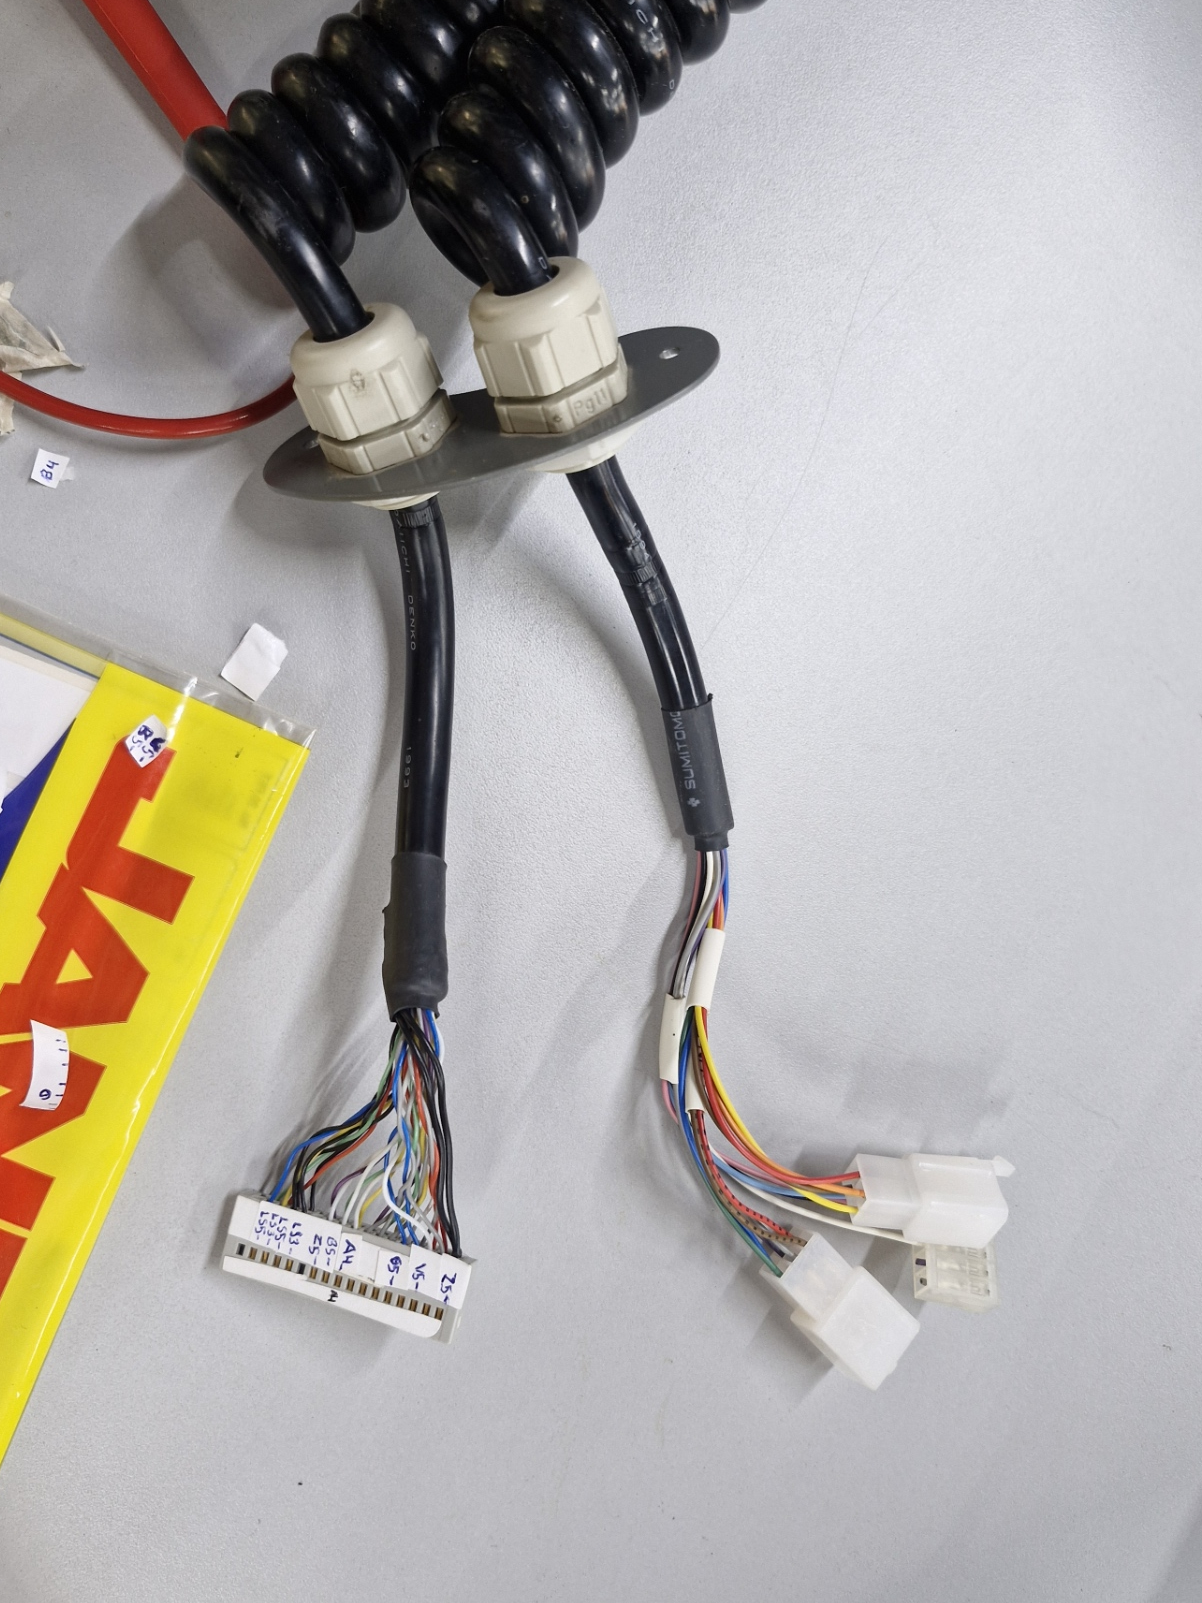
\includegraphics[width=0.95\linewidth]{images/Infraestructura/sdpsegmentos.png}
			\caption[Distribución General del SDP]{\small Organización simétrica de la interfaz: Segmento B (izq.) y Segmento A (der.).}
			\label{fig:distribucion_sdp}
		\end{minipage}
	\end{figure}
	
	
	
	\clearpage
	
	
	\section{Identificación de Componentes y Código de Colores}
	\textbf{Encoders}
	
	Para consolidar el mapeo eléctrico, se presentan a continuación las tablas de correspondencia para cada uno de los cinco encoders del brazo robótico. Este registro es vital para la etapa de interconexión física, dado que la falta de estandarización en el cableado original podría derivar en fallas de alimentación o lectura errática de señales. Todas las señales Z no se conectaron al SDP. 
	
	
	% Encoder 1: Cadera
	\begin{table}[h]
		\centering
		\caption{Mapeo de señales y colorimetría - Encoder 1 (Cadera).}
		\label{tab:encoder_cadera}
		\renewcommand{\arraystretch}{1.5}
		\rowcolors{2}{green!5}{white}
		\begin{tabular}{lccc}
			\toprule
			\textbf{Señal} & \textbf{S. Captación} & \textbf{S. Transmisión} & \textbf{SDP (Pin)} \\ \midrule
			V (Voltaje)    & Amarillo              & N/A                     & N/A                \\
			G (GND)        & Verde                 & N/A                     & N/A                \\
			A (Datos)      & Rojo                  & N/A                     & N/A                \\
			B (Datos)      & Gris                  & N/A                     & N/A                \\
			Z (Índice)     & Azul                  & N/A                     & N/A                \\ \bottomrule
		\end{tabular}
	\end{table}
	
	% Encoder 2: Hombro
	\begin{table}[h]
		\centering
		\caption{Mapeo de señales y colorimetría - Encoder 2 (Hombro).}
		\label{tab:encoder_hombro}
		\renewcommand{\arraystretch}{1.5}
		\rowcolors{2}{green!5}{white}
		\begin{tabular}{lccc}
			\toprule
			\textbf{Señal} & \textbf{S. Captación} & \textbf{S. Transmisión} & \textbf{SDP (Pin)} \\ \midrule
			V (Voltaje)    & Amarillo              & N/A                     & Rojo (16)          \\
			G (GND)        & Verde                 & N/A                     & Gris (14)          \\
			A (Datos)      & Rojo                  & N/A                     & Gris (12)          \\
			B (Datos)      & Gris                  & N/A                     & Amarillo (12)      \\
			Z (Índice)     & Azul                  & N/A                     &  N/A        \\ \bottomrule
		\end{tabular}
	\end{table}
	
	% Encoder 3: Codo
	\begin{table}[h]
		\centering
		\caption{Mapeo de señales y colorimetría - Encoder 3 (Codo).}
		\label{tab:encoder_codo}
		\renewcommand{\arraystretch}{1.5}
		\rowcolors{2}{green!5}{white}
		\begin{tabular}{lccc}
			\toprule
			\textbf{Señal} & \textbf{S. Captación} & \textbf{S. Transmisión} & \textbf{SDP (Pin)} \\ \midrule
			V (Voltaje)    & Amarillo              & N/A                     & Gris (16)          \\
			G (GND)        & Verde                 & N/A                     & Azul (14)          \\
			A (Datos)      & Rojo                  & N/A                     & Morado (10)        \\
			B (Datos)      & Gris                  & N/A                     & Gris (11)          \\
			Z (Índice)     & Azul                  & N/A                     & N/A       \\ \bottomrule
		\end{tabular}
	\end{table}
	
	% Encoder 4: Antebrazo
	\begin{table}[h]
		\centering
		\caption{Mapeo de señales y colorimetría - Encoder 4 (Antebrazo).}
		\label{tab:encoder_antebrazo}
		\renewcommand{\arraystretch}{1.5}
		\rowcolors{2}{green!5}{white}
		\begin{tabular}{lccc}
			\toprule
			\textbf{Señal} & \textbf{S. Captación} & \textbf{S. Transmisión} & \textbf{SDP (Pin)} \\ \midrule
			V (Voltaje)    & Rojo                  & Rojo                    & Rojo (15)          \\
			G (GND)        & Gris                  & Azul                    & Blanco (13)        \\
			A (Datos)      & Azul                  & Verde Claro             & Blanco (9)         \\
			B (Datos)      & Verde                 & Amarillo                & Amarillo (9)       \\
			Z (Índice)     & Amarillo              & Gris                    & N/A        \\ \bottomrule
		\end{tabular}
	\end{table}
	
	% Encoder 5: Muñeca
	\begin{table}[h]
		\centering
		\caption{Mapeo de señales y colorimetría - Encoder 5 (Muñeca).}
		\label{tab:encoder_muneca}
		\renewcommand{\arraystretch}{1.5}
		\rowcolors{2}{green!5}{white}
		\begin{tabular}{lccc}
			\toprule
			\textbf{Señal} & \textbf{S. Captación} & \textbf{S. Transmisión} & \textbf{SDP (Pin)} \\ \midrule
			V (Voltaje)    & Rojo                  & Rojo                    & Blanco (15)        \\
			G (GND)        & Gris                  & Azul                    & Azul (13)          \\
			A (Datos)      & Azul                  & Verde Claro             & Morado (7)         \\
			B (Datos)      & Verde                 & Amarillo                & Blanco (8)         \\
			Z (Índice)     & Amarillo              & Gris                    & N/A         \\ \bottomrule
		\end{tabular}
	\end{table}
	
	\clearpage
	\textbf{Frenos}
	
	% Tabla de Frenos: Hombro y Codo
	\begin{table}[h]
		\centering
		\caption[Mapeo de señales: Frenos B2 y B3]{Mapeo de señales y colorimetría de frenos electromecánicos - Articulaciones B2 (Hombro) y B3 (Codo).}
		\label{tab:mapeo_frenos}
		\renewcommand{\arraystretch}{1.5}
		
		% El color inicia en la fila 2 (la primera de datos), dejando el encabezado blanco
		\rowcolors{2}{green!5}{white} 
		
		\begin{tabular}{lccc}
			\toprule
			% Encabezado sin \rowcolor
			\textbf{ID (Lugar)} & \textbf{S. Captación} & \textbf{S. Transmisión} & \textbf{SDP (Pin)} \\ 
			\midrule
			B2 (Hombro) & Blanco / Blanco & Blanco / Negro & Rosa / Azul \\
			B3 (Codo)   & Blanco / Blanco & Blanco / Negro & Blanco / Negro \\ 
			\bottomrule
		\end{tabular}
	\end{table}
	\textbf{Segmento B}
\begin{table}[h]
	\centering
	\caption[Mapeo SDP: Cara Inferior]{Distribución de señales y colorimetría en la cara inferior del conector SDP (Columna Izquierda del Alzado).}
	\label{tab:sdp_inferior}
	\renewcommand{\arraystretch}{1.5}
	\rowcolors{2}{green!5}{white}
	\begin{tabular}{llcl}
		\toprule
		\textbf{ID Señal} & \textbf{Ubicación} & \textbf{Pin} & \textbf{Color de Conector} \\
		\midrule
		VACÍO & INFERIOR & 1  & VACÍO \\
		LS5   & INFERIOR & 2  & AZUL \\
		LS3   & INFERIOR & 3  & AMARILLO \\
		LS5   & INFERIOR & 4  & NEGRO \\
		LS3   & INFERIOR & 5  & NEGRO \\
		LS1   & INFERIOR & 6  & NA \\
		A1    & INFERIOR & 7  & NA \\
		B5    & INFERIOR & 8  & BLANCO \\
		A4    & INFERIOR & 9  & BLANCO \\
		VACÍO & INFERIOR & 10 & NA \\
		B3    & INFERIOR & 11 & GRIS \\
		A2    & INFERIOR & 12 & GRIS \\
		G5    & INFERIOR & 13 & AZUL \\
		G3    & INFERIOR & 14 & AZUL \\
		V5    & INFERIOR & 15 & BLANCO \\
		V3    & INFERIOR & 16 & GRIS \\
		G1    & INFERIOR & 17 & NEGRO \\
		\bottomrule
	\end{tabular}
\end{table}

\begin{table}[h]
	\centering
	\caption[Mapeo SDP: Cara Superior]{Distribución de señales y colorimetría en la cara superior del conector SDP (Columna Derecha del Alzado).}
	\label{tab:sdp_superior}
	\renewcommand{\arraystretch}{1.5}
	\rowcolors{2}{green!5}{white}
	\begin{tabular}{llcl}
		\toprule
		\textbf{ID Señal} & \textbf{Ubicación} & \textbf{Pin} & \textbf{Color de Conector} \\
		\midrule
		LS1   & SUPERIOR & 18 & NA \\
		LS4   & SUPERIOR & 19 & VERDE \\
		LS2   & SUPERIOR & 20 & ROJO \\
		LS4   & SUPERIOR & 21 & NEGRO \\
		LS2   & SUPERIOR & 22 & NEGRO \\
		VACÍO & SUPERIOR & 23 & VACÍO \\
		A5    & SUPERIOR & 24 & MORADO \\
		B1    & SUPERIOR & 25 & NA \\ % Corregido de 1B a B1 según el plano
		B4    & SUPERIOR & 26 & AMARILLO \\
		A3    & SUPERIOR & 27 & MORADO \\ % Fila de la Muesca Izquierda
		Z2    & SUPERIOR & 28 & VERDE \\
		B2    & SUPERIOR & 29 & AMARILLO \\
		G4    & SUPERIOR & 30 & BLANCO \\
		V4    & SUPERIOR & 31 & ROJO \\
		V2    & SUPERIOR & 32 & ROJO \\
		V1    & SUPERIOR & 33 & NEGRO \\
		G2    & SUPERIOR & 34 & GRIS \\ % Colocado al final para mantener secuencia numérica estricta 18-34
		\bottomrule
	\end{tabular}
\end{table}
	\clearpage
	\section{Consolidación de Datos y Requerimientos de Diseño}
	
	Los registros detallados en las tablas anteriores (ver Tablas \ref{tab:sdp_superior} y \ref{tab:sdp_inferior}) no son únicamente una transcripción del hardware; representan el resultado de un proceso de validación técnica integral. Para garantizar la fiabilidad del sistema de control, se implementó una metodología de pruebas que permitió asegurar la operatividad de cada periférico antes de proceder a la etapa de integración electrónica.
	
	El levantamiento de este inventario técnico y las pruebas de campo asociadas fueron los pilares para establecer las directrices de la PCB de acondicionamiento:
	
	\begin{itemize}
		\item \textbf{Pruebas de Continuidad:} Se realizó una medición de continuidad punto a punto entre las terminales de los tres niveles jerárquicos (\textit{Captación, Transmisión y SDP}). Este procedimiento permitió confirmar la integridad del arnés original del robot y asegurar que el mapeo de señales fuera 100\% fiel a la realidad física del sistema.
		\item \textbf{Validación de Componentes:} Mediante la activación manual y medición de señales, se comprobó el correcto funcionamiento de los sensores de límite, encoders y frenos. Esta certeza técnica redujo significativamente el riesgo de fallas críticas durante las pruebas de energización de la nueva interfaz.
		\item \textbf{Definición de Interfaz:} La identificación precisa de los pines en la terminal de $2 \times 17$ (Segmento B) dictó las especificaciones de conectividad mecánica y niveles lógicos de voltaje que la PCB debe procesar para proteger la integridad del microcontrolador y los sensores.
	\end{itemize}
	
	De este modo, la información consolidada en este capítulo constituye la base técnica necesaria para la transición de la infraestructura original hacia el nuevo sistema de control electrónico personalizado.
	
	\subsection{Pruebas hechas a los finales de carrera}
	El circuito implementado representa un final de carrera (representado por el switch SPST) configurado en un arreglo de \textbf{Pull-Down}. Cuando el switch no está presionado (NC - Normal Cerrado, como se muestra en la imagen del Proteus), actúa como un cortocircuito que conecta la fuente de 5V directamente al nodo de salida \verb|out| y a través de la resistencia \verb|R1| $1k \Omega$ a GND. En este estado, la medición en \verb|out| y a través de \verb|R1| es de 5V directos de la fuente, indicando un '1' lógico estable. La resistencia limita la corriente extraída de la fuente para que el microcontrolador solo lea el voltaje sin causar un cortocircuito.
	
	Al presionar el final de carrera, el switch se abre, desconectando la fuente de 5V del nodo. En ese instante, la resistencia \verb|R1| jala el potencial del nodo de salida hacia tierra (0V), asegurando que el microcontrolador lea un '0' lógico estable y eliminando el estado flotante que ocurriría sin ella. El voltímetro en la simulación confirma que la diferencia de potencial a través de la resistencia es de 5V constantes mientras el switch está NC, validando eléctricamente la configuración de Pull-Down y el estado 'NO Presionado'.
	
	\begin{figure}[h]
		\centering
		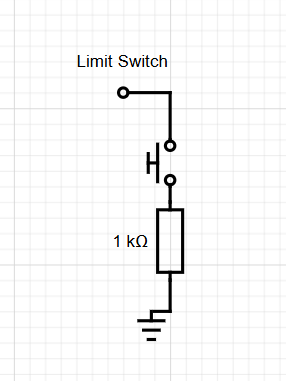
\includegraphics[width=0.4\linewidth]{images/encoders/lsdiagrama}
		\caption{Diagrama de conexión del final de carrera. Se colocó un resistor pull down.}
		\label{fig:lsdiagrama}
	\end{figure}
	
	
	
	\begin{figure}[htbp]
		\centering
		% Título del bloque
		{\large \textbf{Validación de Estados del Limit Switch}} \\[0.4cm]
		
		% --- FILA 1: Simulaciones en Proteus ---
		\begin{minipage}{0.48\textwidth}
			\centering
			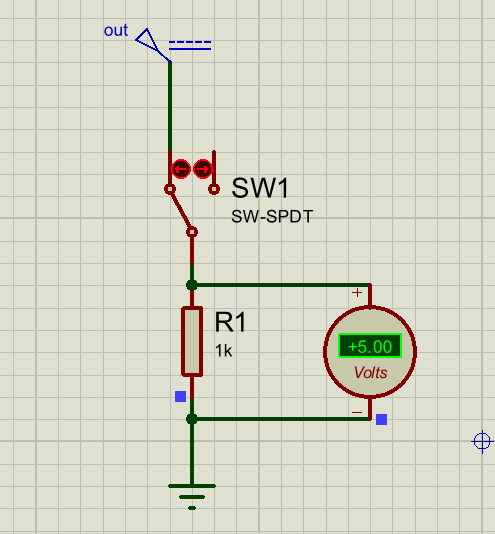
\includegraphics[width=\linewidth]{images/Infraestructura/nc.png}
			\caption[Simulación en proteus del final de carrera no presionado.]{Simulación Proteus: El final de carrera no se ha presionado. Se registran 5V directos.}
			\label{fig:NC}
		\end{minipage}
		\hfill
		\begin{minipage}{0.48\textwidth}
			\centering
			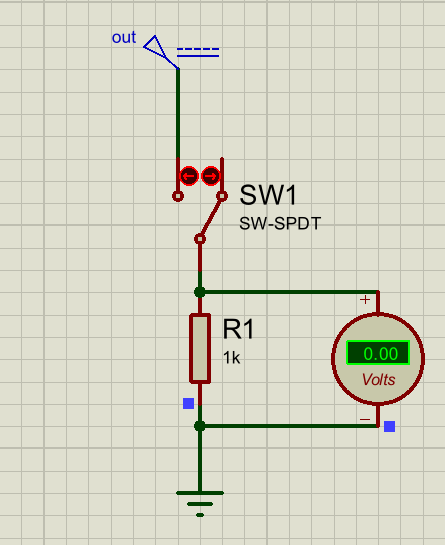
\includegraphics[width=\linewidth]{images/Infraestructura/ncabirer.png}
			\caption[Simulación en proteus del final de carrera simulado]{Simulación Proteus: El final de carrera se presionó. Salida a 0V por Pull-Down.}
			\label{fig:LSabierto}
		\end{minipage}
		
		\vspace{0.6cm} % Espacio vertical entre filas
		
		% --- FILA 2: Mediciones de Voltaje ---
		\begin{minipage}{0.48\textwidth}
			\centering
			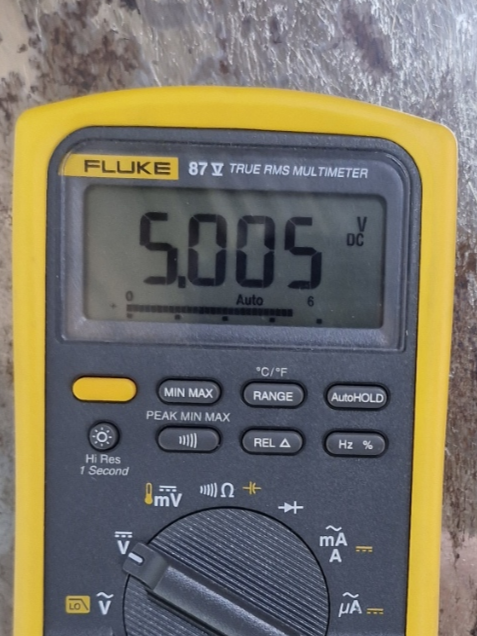
\includegraphics[width=\linewidth]{images/Infraestructura/5vls.png}
			\caption{Voltaje leído cuando el final de carrera no está presionado (5V).}
			\label{fig:voltaje_nc}
		\end{minipage}
		\hfill
		\begin{minipage}{0.48\textwidth}
			\centering
			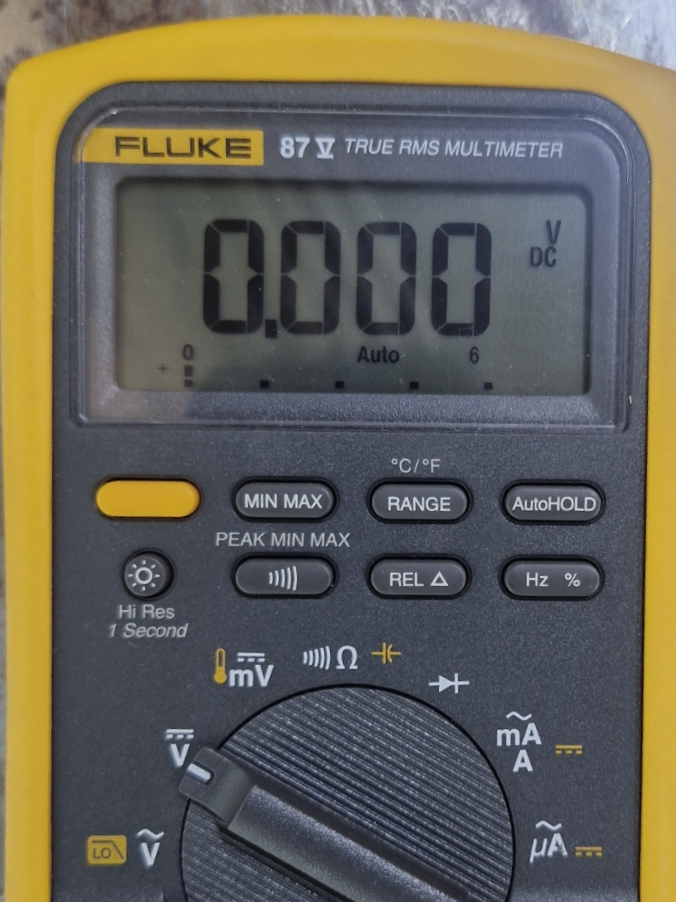
\includegraphics[width=\linewidth]{images/Infraestructura/vsss.png}
			\caption{Voltaje leído cuando el final de carrera está presionado (0V).}
			\label{fig:voltaje_presionado}
		\end{minipage}
		
		\vspace{0.3cm}
	\end{figure}\clearpage
	
	\begin{figure}[htbp]
		\centering
		% --- Imagen Izquierda: Encoders ---
		\begin{minipage}{0.48\textwidth}
			\centering
			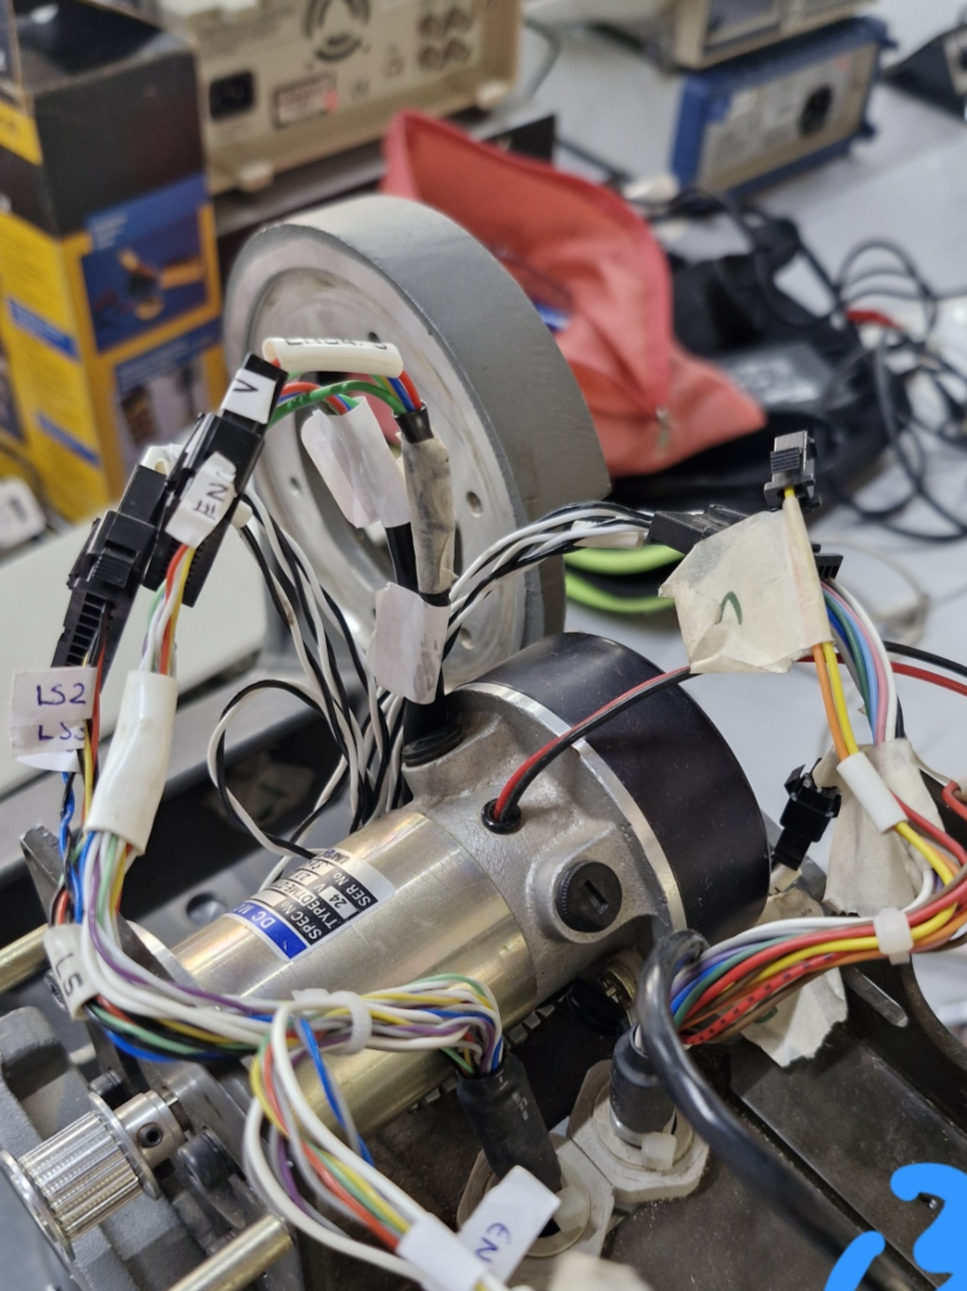
\includegraphics[width=\linewidth]{images/Infraestructura/et.png}
			\caption{Etiquetado realizado en el segmento de transmisión de los encoders.}
			\label{fig:etiquetado_encoders}
		\end{minipage}
		\hfill % Espacio elástico entre las dos minipages
		% --- Imagen Derecha: Finales de Carrera ---
		\begin{minipage}{0.48\textwidth}
			\centering
			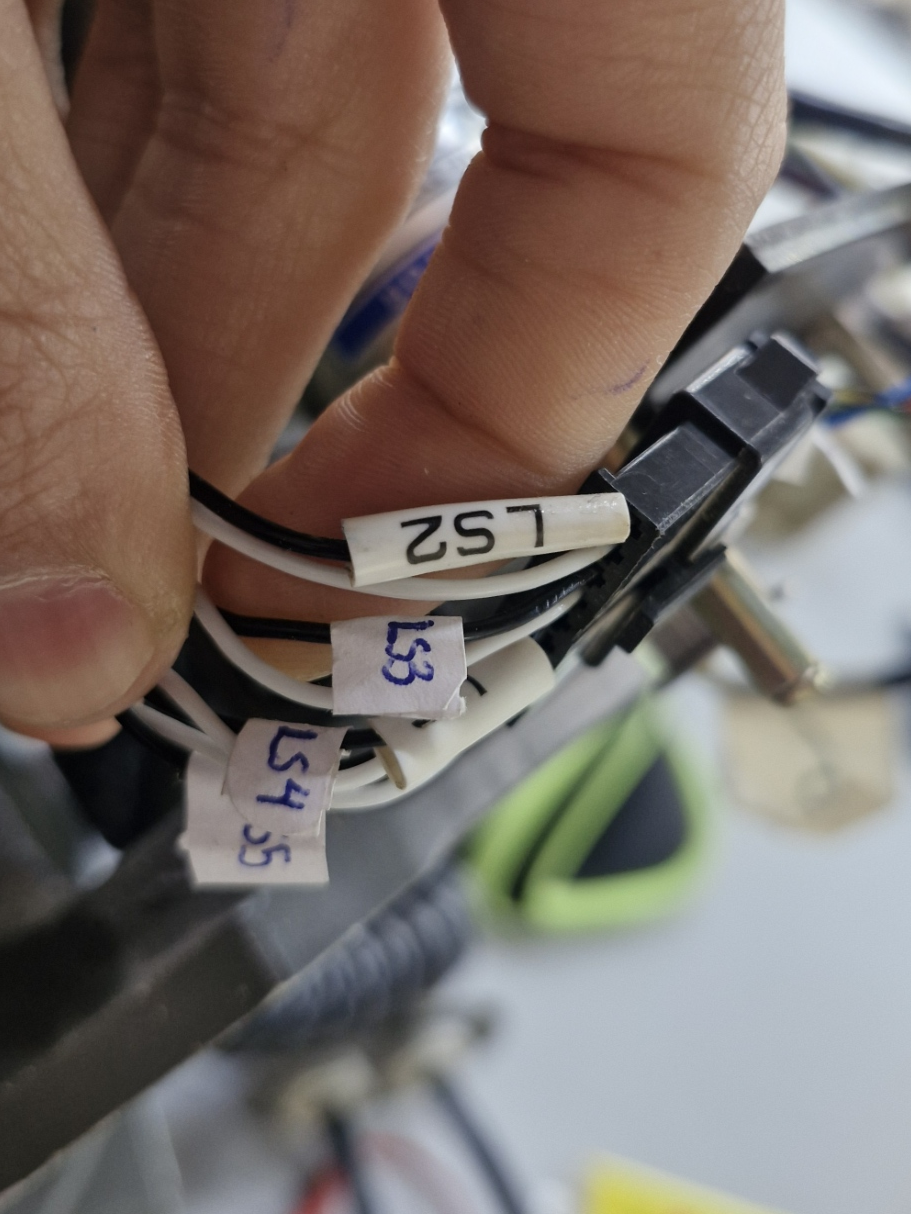
\includegraphics[width=\linewidth]{images/Infraestructura/kset.png}
			\caption{Etiquetado en los finales de carrera.}
			\label{fig:etiquetado_ls}
		\end{minipage}
	\end{figure}
	
	\subsection{Sistema de Control de Frenado Electromecánico}
	
	El brazo robótico Mitsubishi Move Master EX integra frenos electromecánicos en sus articulaciones principales (Hombro y Codo) para evitar colapsos por gravedad ante la ausencia de energía. Estos dispositivos operan a una tensión nominal de \textbf{12V DC}. 
	
	Debido a que el microcontrolador opera a niveles lógicos de 5V y no posee la capacidad de manejar la corriente requerida por las bobinas de los frenos, se diseñó una etapa de conmutación utilizando transistores de potencia \textbf{MOSFET IRFZ44N}.
	
	\subsubsection{Configuración del Driver de Potencia}
	
	La implementación se basa en una configuración de conmutación de lado bajo (\textit{low-side switch}). En este diseño:
	\begin{itemize}
		\item Los frenos mantienen una conexión directa a la línea positiva de \textbf{+12V}.
		\item El terminal de tierra (GND) de cada freno se conecta al \textit{Drain} del MOSFET.
		\item El MOSFET actúa como un \textbf{interruptor electrónico}, cerrando el circuito hacia el GND común del sistema únicamente cuando recibe una señal \texttt{HIGH} en su terminal de \textit{Gate} desde el Arduino Mega.
	\end{itemize}
	
	Esta arquitectura permite un aislamiento efectivo entre la etapa de potencia y la lógica de control, garantizando una respuesta rápida para la liberación de los ejes.
	
	\begin{table}[h!]
		\centering
		\renewcommand{\arraystretch}{1.5}
		\caption{Especificaciones técnicas de la etapa de frenado.}
		\label{tab:especificaciones_frenos}
		\begin{tabularx}{\textwidth}{|X|c|c|c|}
			\hline
			\rowcolor{green!20}
			\textbf{Componente} & \textbf{Señal de Control} & \textbf{Voltaje de Carga} & \textbf{Configuración} \\ \hline
			MOSFET IRFZ44N (A1) & Pin 14 (Hombro) & 12V & Interruptor GND \\ \hline
			MOSFET IRFZ44N (B1) & Pin 15 (Codo)   & 12V & Interruptor GND \\ \hline
		\end{tabularx}
	\end{table}
	
	\begin{figure}[h!]
		\centering
		% Primera imagen: Conexión del freno
		\begin{minipage}{0.45\textwidth}
			\centering
			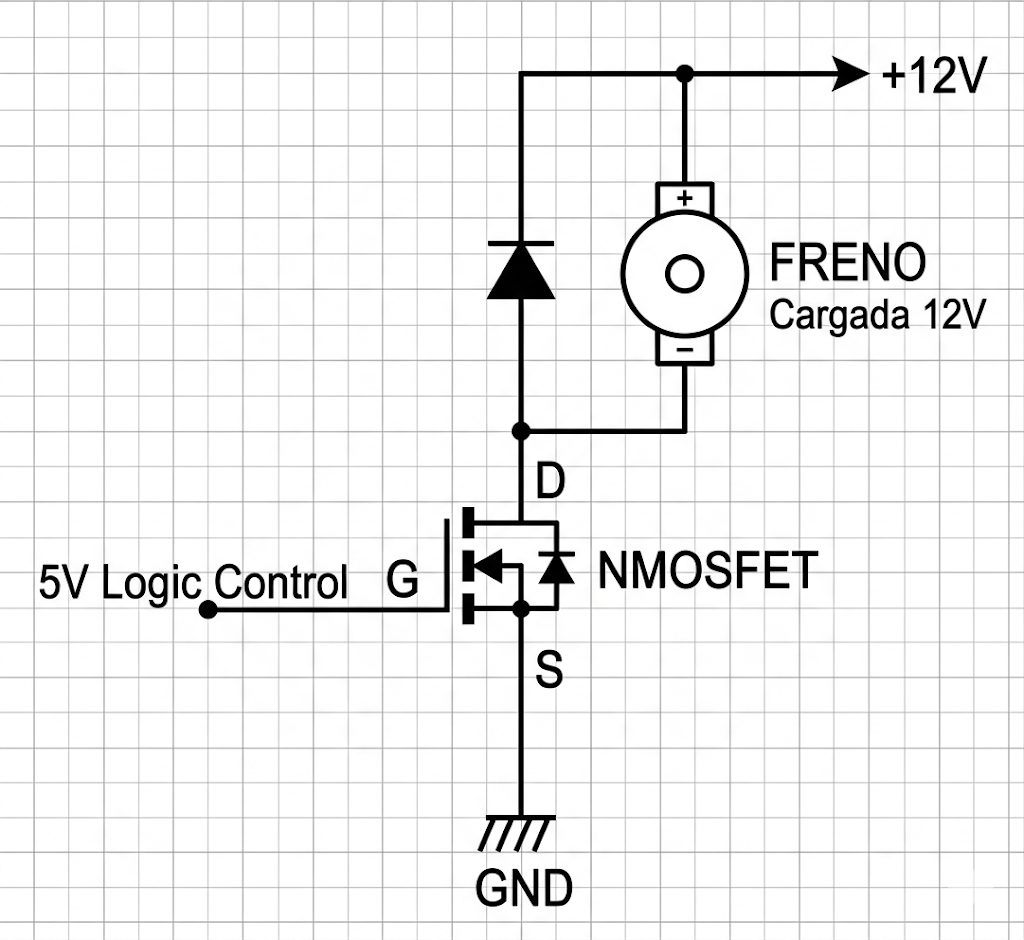
\includegraphics[width=\linewidth]{images/encoders/tarjetaFrenos1}
			\caption{Conexión del freno.}
			\label{fig:tarjetafrenos1}
		\end{minipage}
		\hfill % Espacio entre imágenes
		% Segunda imagen: Especificaciones de motores
		\begin{minipage}{0.45\textwidth}
			\centering
			% Nota: Se recomienda copiar esta imagen a tu carpeta de proyecto
			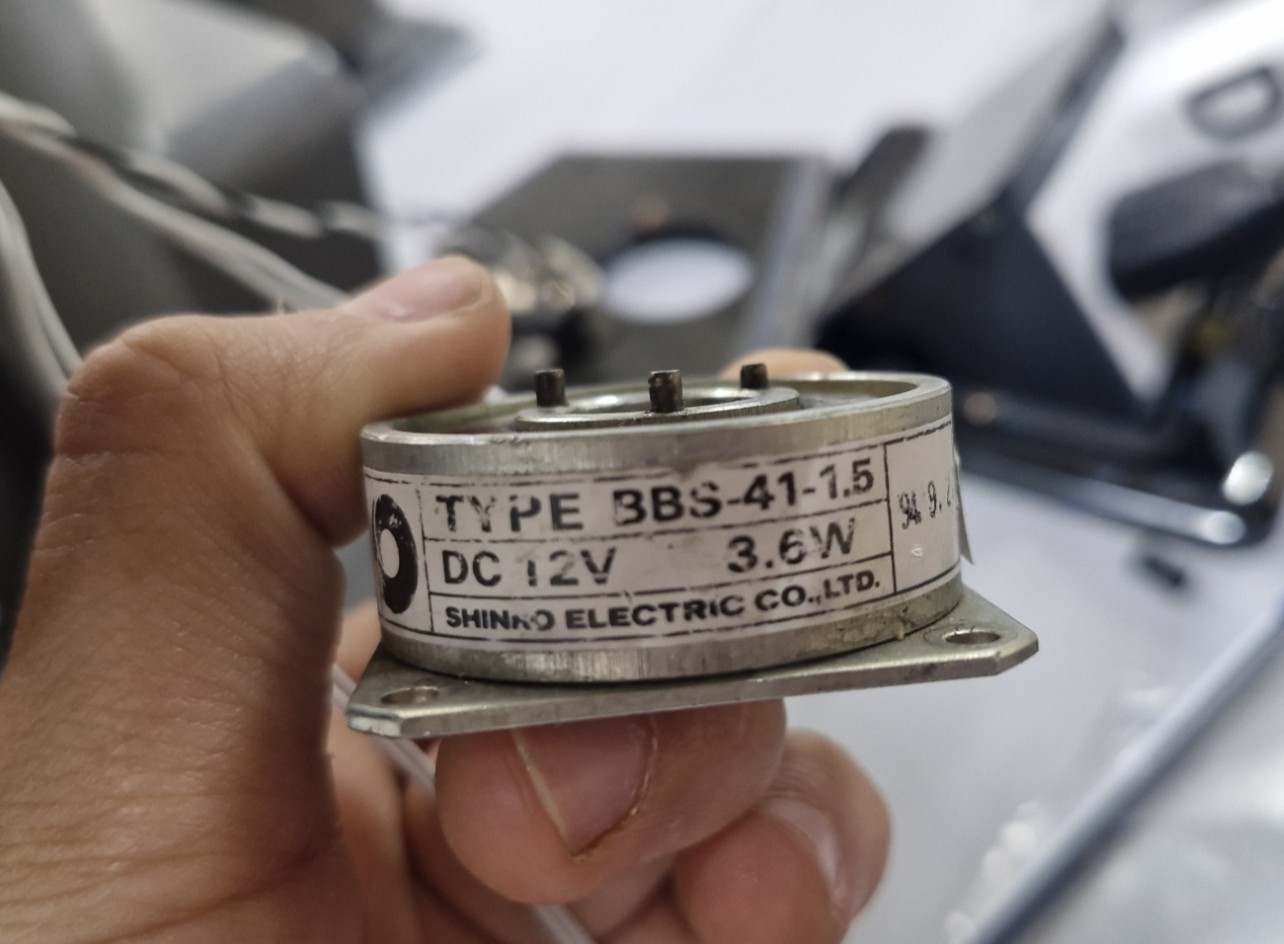
\includegraphics[width=\linewidth]{images/encoders/especificaciones} 
			\caption{Especificaciones de los motores (12 V / 3.6 W).}
			\label{fig:especificaciones_motores}
		\end{minipage}
	\end{figure}
	
	\begin{resultadosFase}
		\begin{itemize}
			
			\item \textbf{Mapeo Integral:} Identificación y documentación del 100\% de la pinout de la interfaz SDP (34 pines), resolviendo la incertidumbre del código de colores original.
			\item \textbf{Validación Eléctrica:} Confirmación de la operatividad de los 5 encoders incrementales y los frenos electromecánicos de los ejes J2 y J3. Se muestran los resultados en el siguiente capítulo.
			\item \textbf{Seguridad Mecánica:} Verificación funcional de los 5 \textit{limit switches}, garantizando una respuesta lógica binaria (0-5V) para la protección del brazo.
			\item \textbf{Base de Diseño:} Definición de los requerimientos de impedancia y niveles lógicos necesarios para la transición a la etapa de diseño de la PCB de acondicionamiento.
		\end{itemize}
	\end{resultadosFase}
